As I explained in Section~\ref{llm} of the background and Section~\ref{llmsforcoevolution} of the state of the art, LLMs are widely explored in Model-Driven Engineering and Software Engineering, but no existing study evaluated the LLMs capabilities 
to support developers in the problem of metamodels and code co-evolution. 
In this chapter, I present a novel approach to mitigate the challenge of metamodel evolution impacts on the code using LLMs (Challenge \Circled{\hyperref[C3]{C3}}). 
%Chatgpt as LLM 
Our approach is based on prompt engineering, where we design and generate natural language prompts to best co-evolve the impacted code due to the metamodel evolution. I first explain how a prompt template is structured, then how I investigated the usefulness of this template structure. 

  Section \ref{ch3_example} presents a motivating example to illustrate the problem of metamodels and code co-evolution. Section \ref{ch3_appraoch} presents our approach for generating prompts and details the prototype implementation.  Section \ref{ch3_evaluation} details our followed methodology in this empirical study. This section assesses the usefulness of my approach and compares ot to IDE quick fixes as a baseline. Section \ref{ch3__results} reports on the obtained results and discusses threats to validity. Finally, Section \ref{ch3_conclu} concludes this chapter. 

\section{Motivating example}
\label{ch3_example}


%To have an overview of the challenge we work on, 
To illustrate the adressed challenge, let us have an example. 
Figure \ref{fig: BMM} shows an excerpt of the  version ~0.9.0 of "Modisco Discovery Benchmark" metamodel. %\footnote{\url{https://git.eclipse.org/r/plugins/gitiles/modisco/org.eclipse.modisco/+/refs/tags/0.12.1/org.eclipse.modisco.infra.discovery.benchmark/model/benchmark.ecore}}.
Modisco is an academic initiative project implemented in the Eclipse platform that has evolved numerous times in the past to support the development of model-driven tools, reverse engineering, verification, and transformation of existing software systems \cite{bruneliere2010modisco,bruneliere2014modisco}.
%consisting of 10 classes in the version of~0.9.0.
Figure \ref{fig: BMM} illustrates  some of the domain concepts \textbf{Discovery}, \textbf{Project}, and \textbf{ProjectDiscovery}  used for the discovery and reverse engineering of an existing software system. 
From these metaclasses, a first code API is generated, containing Java interfaces and their implementation classes, a factory, a package, etc. %(details of created files in table \ref{table: locationofMMelemen}). 
Listing \ref{lis:Modisco_Code_API_V1} shows a snippet of the generated Java interfaces and classes from the metamodel in Figure \ref{fig: BMM}. 

The generated code API is further enriched by the developers with additional code functionalities in the "Modisco Discovery Benchmark" project and its dependent projects as well.
For instance, by implementing the methods defined in metaclasses and advanced functionalities in new classes.
% (\eg language services, tooling, \dots).
Listing \ref{lis:Modisco_Code_External_V1} shows the two classes \texttt{Report} and \texttt{JavaBenchmarkDiscoverer} of the additional code ({\small\boxed{Line~4,8}} in the same project "Modisco Discovery Benchmark" and in another dependent project, namely the "Modisco Java Discoverer Benchmark" project).
%, namely the classes \texttt{CDOProjectDiscoveryImpl} and \texttt{JavaBenchmarkPackageImpl}. 
%
%One of the dependent projects on the Modisco discovery benchmark metamodel is Java Benchmark Discoverer. From this project, as an example, we select 3 classes shown in Listing \ref{lis:Modisco_Code_External_V1}. 
%
%In particular, the classes \texttt{CDOProjectDiscoveryImpl} and \texttt{JavaBenchmarkPackageImpl}, and \texttt{JavaDiscoveredProjectImpl}, which handles information and statistics about CDO and Java project. 
%
%the class \textit{CDOProjectDiscoveryImpl} gives information and statistics about CDO project Discovery. 
%Another dependent class \textit{JavaBenchmarkPackageImpl} that creates and initializes the package' methods %for Package models
%( or Benchmark models ? non). The last class is
%\textit{JavaDiscoveredProjectImpl} that contains different information and statistics about java discovered project. 
%The method \textit{initializePackageContents} (line 12) retrieves a \textit{ProjectDiscovery} instance to initialize the classes of the Java Benchmark Package. The method \textit{eBaseStructuralFeatureID} (line 24) returns the structural identifier of the feature relying on the type of its class.  
%
%From version 0.9.0 to 0.11.0, 
In version~0.11.0, the "Modisco Discovery Benchmark" metamodel evolved with several significant changes, among which the following impacting changes: \emph{1)} Renaming the property \texttt{DicoveryDate} of the class  \texttt{JavaBenchmarkDiscoverer} to \texttt{DiscoveryDate}, and \emph{2)} Moving the property \emph{discoveryTimeInSeconds} from metaclass \texttt{Discovery} to \texttt{DiscoveryIteration}.

%To analyze the consequences of the metamodel evolution on the additional code, we track the impacts of the following metamodel changes:
%\begin{enumerate}%[noitemsep,nolistsep]



%\item Pulled the reference \textit{discoveries} from metaclass \texttt{DiscoveredProject} to \texttt{Benchmark}.
\begin{comment}
	
	
	\begin{itemize}
		\item \emph{1)} Renaming the property \texttt{DicoveryDate} of the class  \texttt{JavaBenchmarkDiscoverer} to \texttt{DiscoveryDate}. % and \texttt{DiscoveredProject}.
		
		\item \emph{2)} Moving the property \emph{discoveryTimeInSeconds} from metaclass \texttt{Discovery} to \texttt{DiscoveryIteration}. 
	\end{itemize} %\DK{maybe choose another rename and move ? averageSaveTimeInSeconds ?}
\end{comment}

\begin{figure}
	
	\centering
	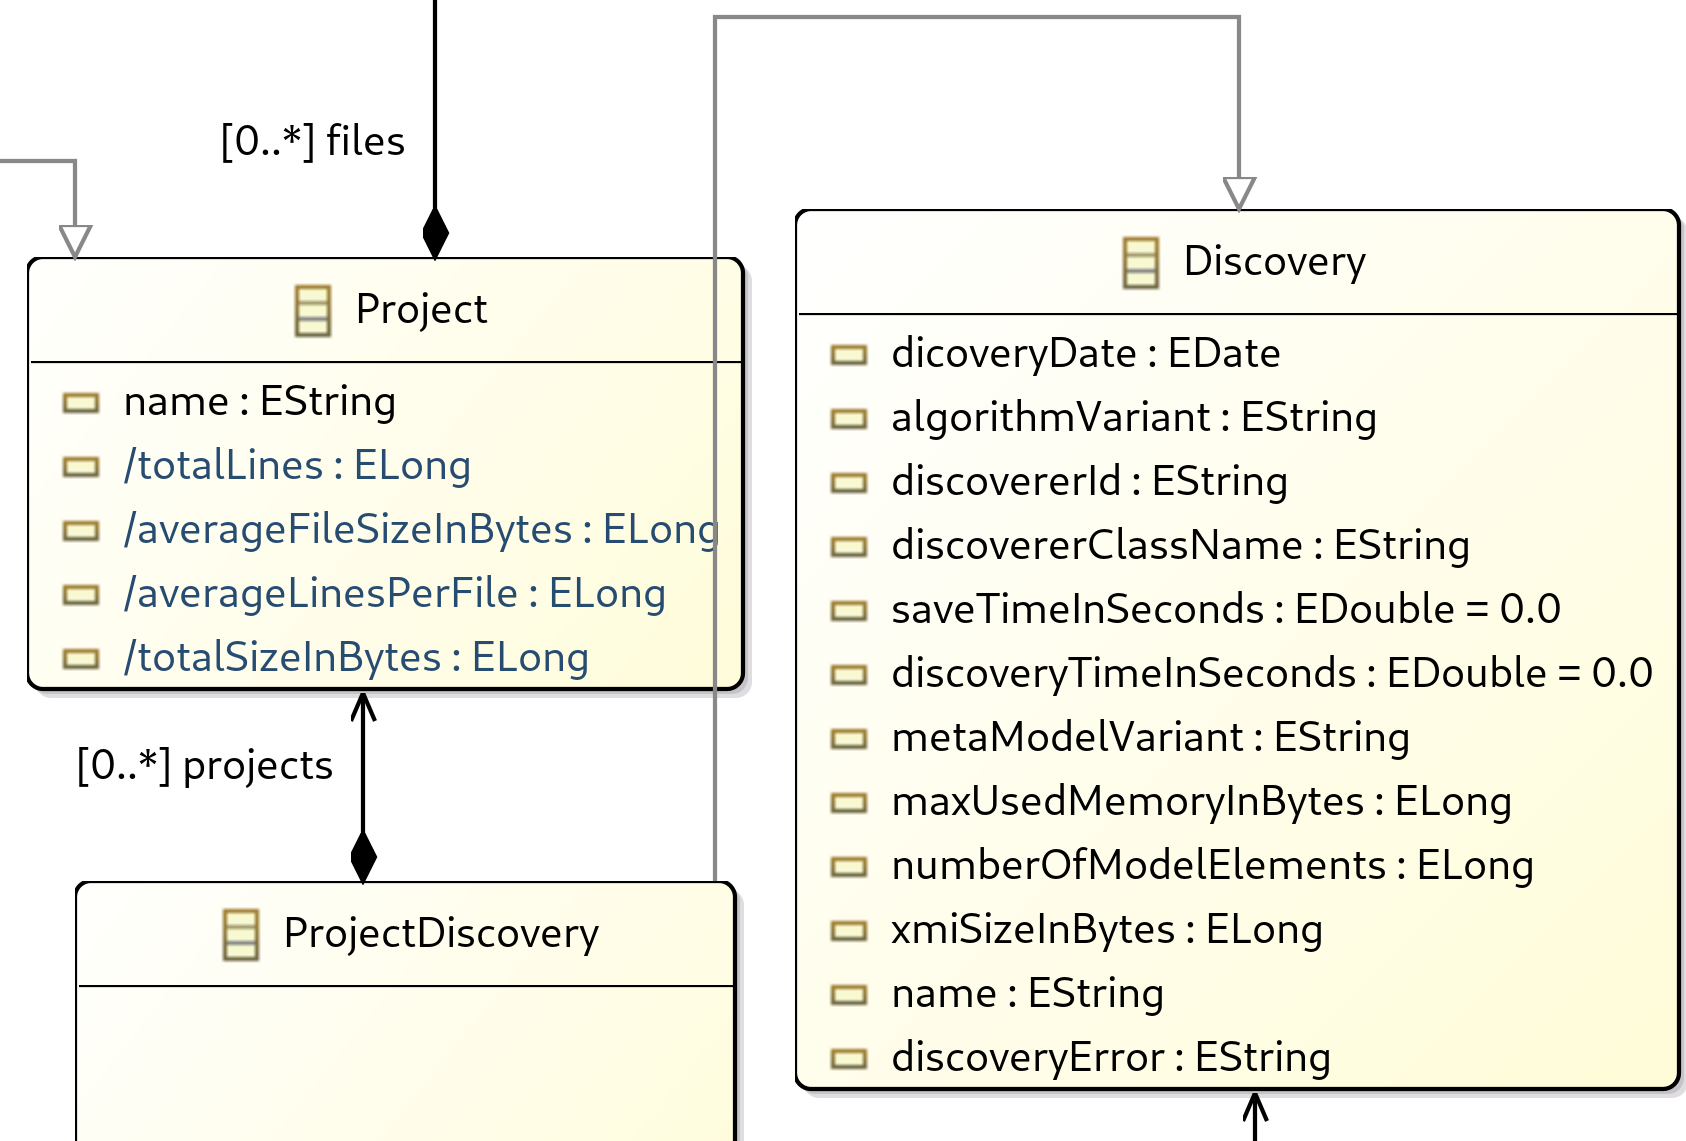
\includegraphics[width=0.55\textwidth]{./pics/chapter3pics/example.PNG}
	\caption{Excerpt of Modisco Benchmark metamodel in version 0.9.0.}
	\label{fig: BMM}
	%\vspace{-5mm}
\end{figure}



After applying these modifications, the code of Listing \ref{lis:Modisco_Code_API_V1} is re-generated from the evolved version of the metamodel, which impacts the existing additional code depicted in Listings \ref{lis:Modisco_Code_External_V1}. 

\begin{lstlisting}[language=Java,breaklines=true,mathescape,literate={\-}{}{0\discretionary{-}{}{}},caption=Excerpt of the generated code in org.eclipse.modisco.infra.discovery.benchmark.,label={lis:Modisco_Code_API_V1}]
	//Discovery Interface
	public interface Discovery extends EObject {
		double getTotalExecutionTimeInSeconds();
		void setTotalExecutionTimeInSeconds(double value);
		...
	}
	//Project Interface
	public interface ProjectDiscovery extends Discovery {...}
	//DiscoveryImpl Class
	public class DiscoveryImpl extends EObjectImpl implements Discovery {
		public double getTotalExecutionTimeInSeconds() {...}
		public void setTotalExecutionTimeInSeconds(double totalExecTime) {...}
		...
	}
\end{lstlisting}
%xleftmargin=0.2cm,xrightmargin=0cm,framexleftmargin=+6pt,frame=single,
\begin{lstlisting}[language=Java,breaklines=true,mathescape,literate={\-}{}{0\discretionary{-}{}{}},caption=Excerpt of the additional code V1.,label={lis:Modisco_Code_External_V1}]
	
	public class Report {
		...
		discovery.(*\ul{setDiscoveryTimeInSeconds}*)(...);
	}
	
	public class JavaBenchmarkDiscoverer extends AbstractModelDiscoverer<IFile> {
		...
		discovery.(*\ul{setDicoveryDate}*)(new Date());
		...
	} 
\end{lstlisting}


%%%%%%%%%%%%%%%%%%%%%%%%%%%%%%%%%%%%%%%%%%%%%%%%%%%%%%%%%%%
%%                   Now the evolved code                %%
%%%%%%%%%%%%%%%%%%%%%%%%%%%%%%%%%%%%%%%%%%%%%%%%%%%%%%%%%%%
\setulcolor{green} 
%\setstcolor{green}
%\setstcolor{green}
%,xleftmargin=0.2cm,,xrightmargin=-0cm,framexleftmargin=+6pt,frame=single
\begin{lstlisting}[language=Java,breaklines=true,mathescape,literate={\-}{}{0\discretionary{-}{}{}},caption=Excerpt of the additional code V2.,label={lis:Modisco_Code_External_V2}]
	
	public class Report {
		...
		discovery.(*\ul{getIterations().get(0).}*) 
		(*\ul{setDiscoveryTimeInSeconds}*)(...);
		...
	}
	
	public class JavaBenchmarkDiscoverer extends AbstractModelDiscoverer<IFile> {
		...
		discovery.(*\ul{setDiscoveryDate}*)(new Date());
		...
	}
\end{lstlisting}




The resulting errors in the original code in version 0.9.0 are underlined in red in Listing \ref{lis:Modisco_Code_External_V1}. Listing \ref{lis:Modisco_Code_External_V2} presents the final result of the manual developer's co-evolution in version 0.11.0. The co-evolved code is underlined in green. 
% Expected co-evolution ?
The changes \textit{rename} of the property \textit{ DicoveryDate} and the \textit{move} of the property \emph{discoveryTimeInSeconds} impact their usages ({\small\boxed{Line~4,8}} in Listing~\ref{lis:Modisco_Code_External_V1}). The impact of renaming \textit{ DicoveryDate} is co-evolved by replacing \textit{setDicoveryDate} by \textit{setDiscoveryDate}. The impact of moving the property \emph{discoveryTimeInSeconds} is co-evolved by extending the call path of the method \emph{setDiscoveryTimeInSeconds} through the reference \textit{iterations} by calling the method \textit{getIterations} and getting the first element of the returned list of DiscoveryIteration objects.

%The above examples show the importance of correctly matching the different code usages of the generated code with the metamodel evolution changes to co-evolve them with the appropriate resolutions.  
Developers unfortunately manually co-evolve the code, which is tedious, error-prone, and time-consuming. 
One help developers get is from the IDE and the provided quick fixes. For example, when using Eclipse quick fixes to co-evolve these errors, it suggests creating the method \texttt{setDiscoveryTimeInSeconds} in the class \texttt{Discovery}, which does not meet the required co-evolutions shown in Listing~\ref{lis:Modisco_Code_External_V2}.

With the ever-growing popularity and promising results of LLMs, a developer can prompt an LLM to suggest a co-evolution. 
For example, 
%To motivate more our work, 
we asked ChatGPT to co-evolve the error resulted from moving the property \emph{discoveryTimeInSeconds} by giving the erroneous code ({\small\boxed{Line~4}} in Listing~\ref{lis:Modisco_Code_External_V1})  with the message of the error taken from eclipse Problems window. This is the first intuition when using ChatGPT because the developer does not know necessarily the metamodel change causing the error and finding it due to the abstraction gap is a tedious and error-prone task. Figure \ref{fig: chatgptanswer} shows that ChatGPT proposes to create a method named \emph{setDiscoveryTimeInSeconds} in the class \emph{Discovery}, which is totally wrong because it does not fit the causing change. 

Our Hypothesis is that the LLM fails because our problem is more complex than simply repairing a code error. It must understand the original impacting metamodel change traced to the code error, as well as the abstraction gap between the two artefacts of metamodels and code. After improving the prompt, \LLM succeeded to give the right resolution as show in Figure \ref{fig: chatgptimprovedanswer}.
Our vision is that this contextual rich information must be injected in the prompt.
Thus, the quality of the prompt is a key for the LLM to solve this problem of metamodels and code co-evolution. %Indeed, it is a hard problem due to the abstraction gap between the two artefacts of metamodels and code. This context should be part of the prompt as well as the impacting metamodle change that must be traced to the code error. 

%by giving only the errouneous ({\small\boxed{Line~4}} in Listing~\ref{lis:Modisco_Code_External_V1}). Chatgpt answer in this case was totaly wrong. Thus, we injected the change information in the request and asked Chatgpt to coevolve the same error. Figure \ref{fig: chatgptanswer} shows that even adding the change information did not help chatgpt to find the right resolution.
%
The next section presents our contribution for a contextualized information rich prompts-based co-evolution of metamodel and code using LLMs.  


\begin{figure}[t]
	\centering
	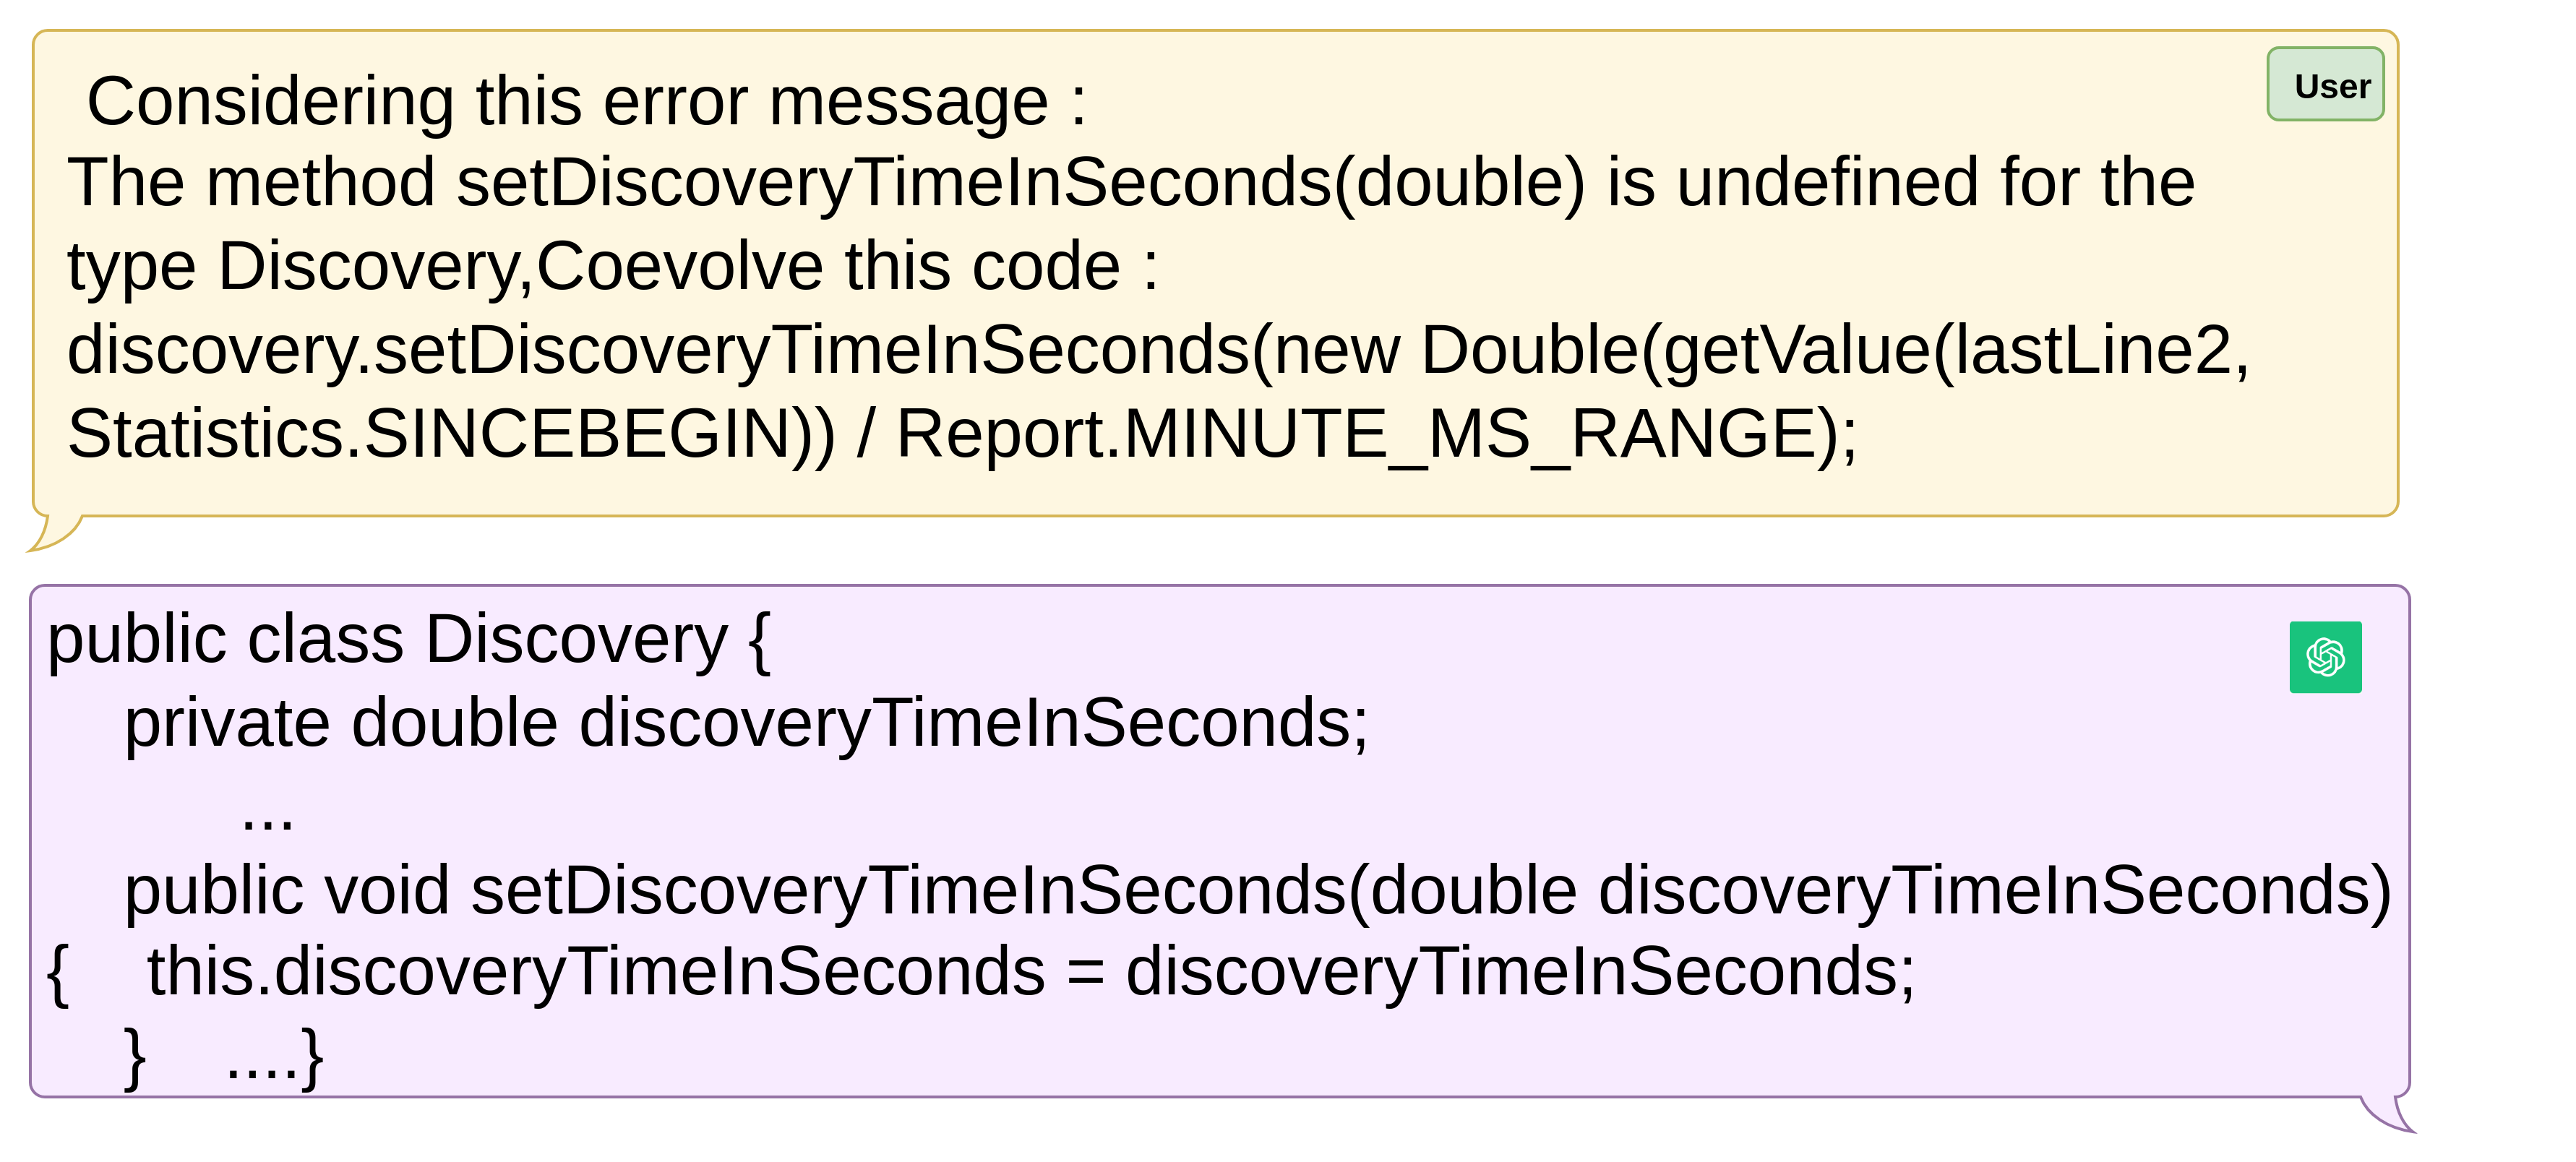
\includegraphics[width=0.48\textwidth]{./pics/chapter3pics/chatgptprimitiveanswer.png}
	\caption{ChatGPT primitive answer to the naive prompt.}
	\label{fig: chatgptanswer}
	%\vspace{-5mm}
\end{figure}

\begin{figure}[t]
	\centering
	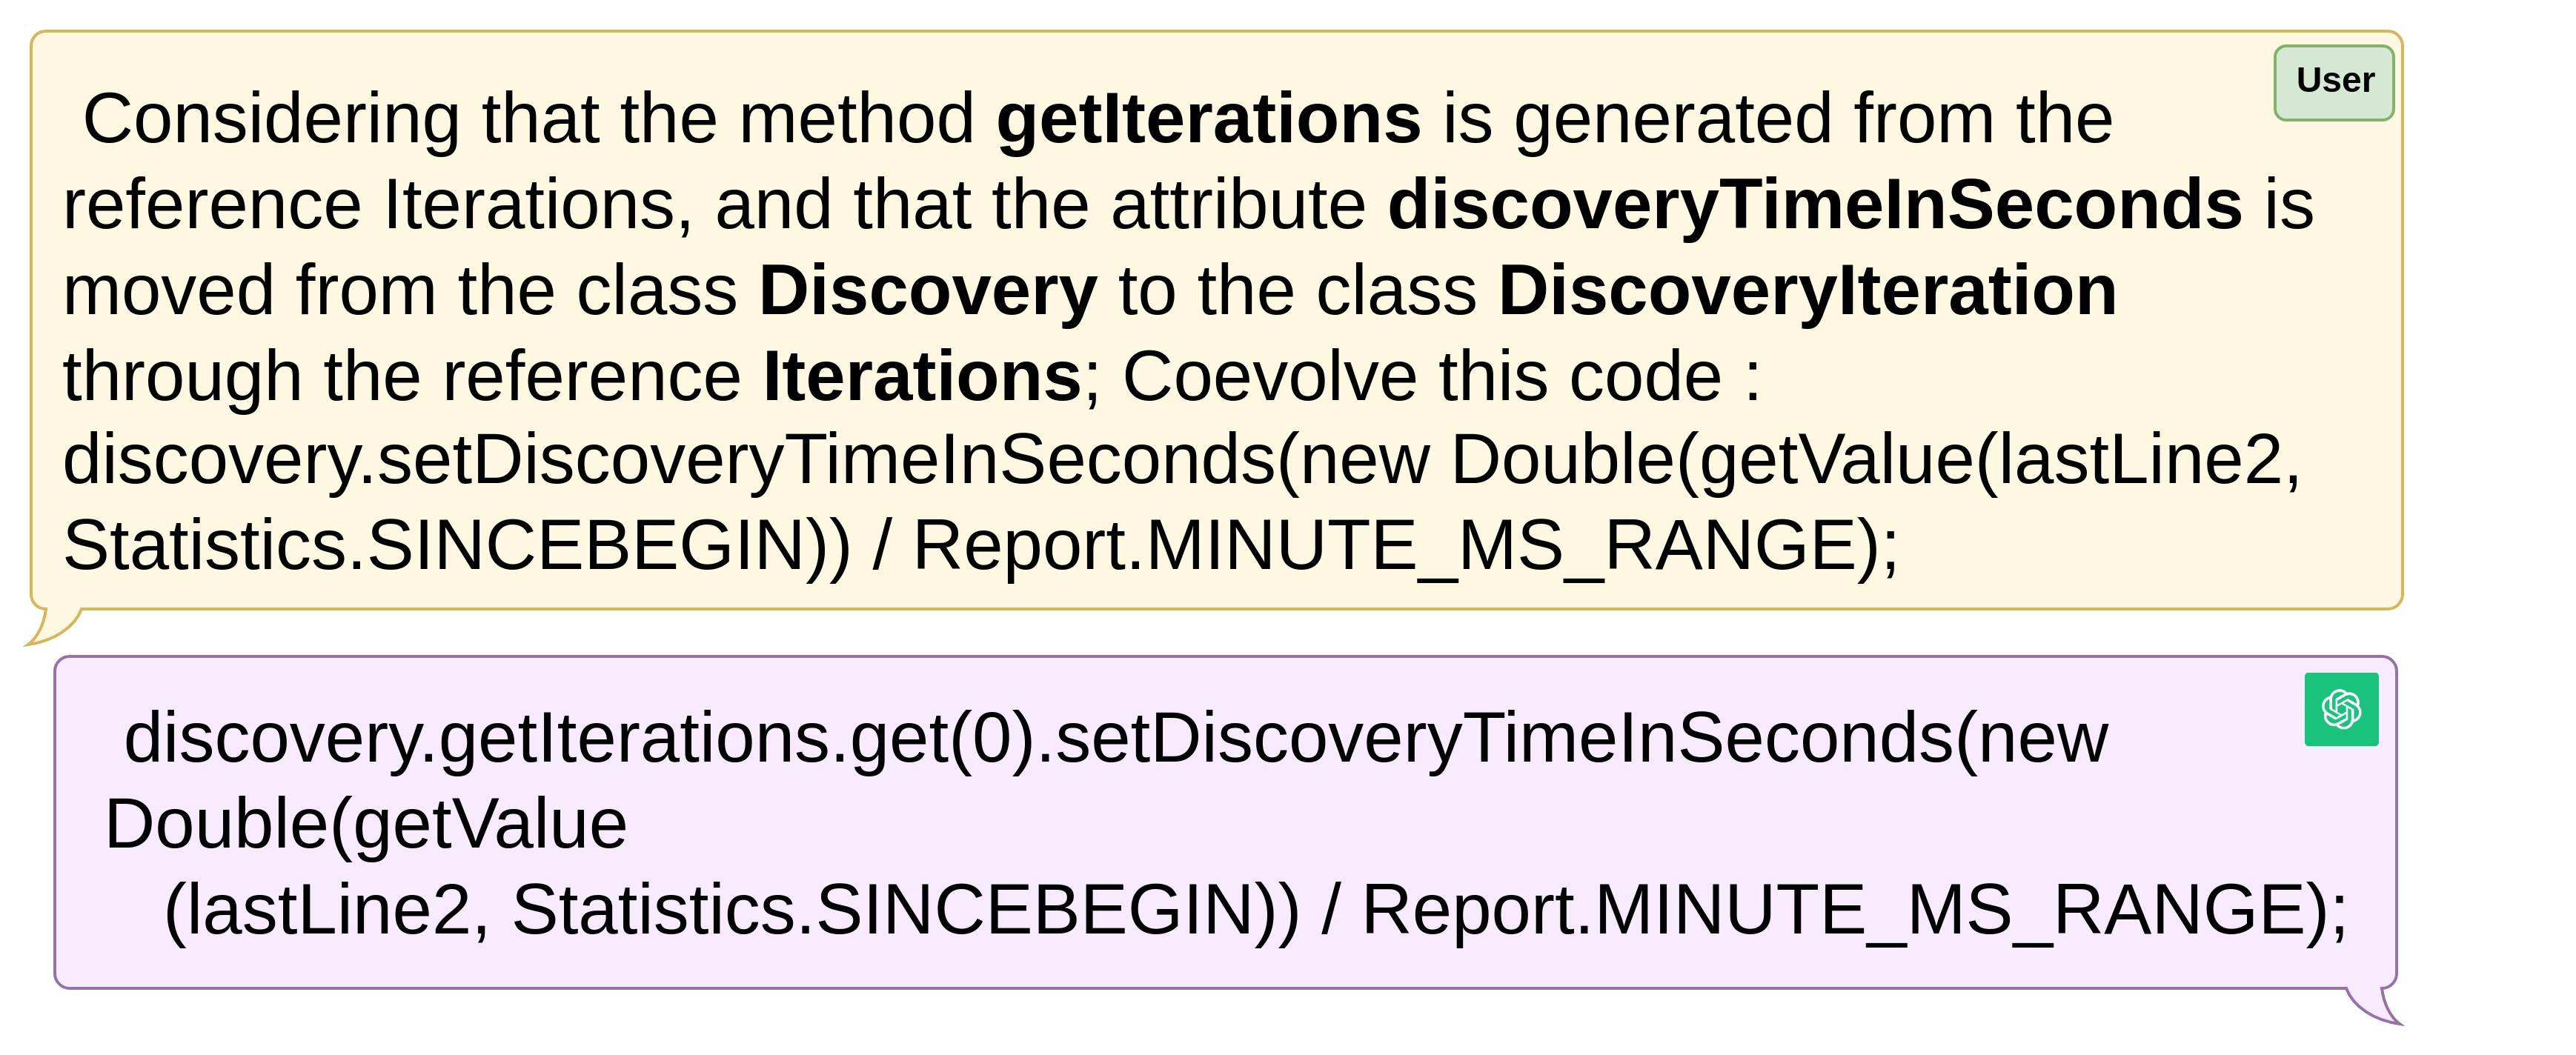
\includegraphics[width=0.48\textwidth]{./pics/chapter3pics/chatgptimprivedanswer.png}
	\caption{\LLM improved answer with the enriched prompt with contextual information.}
	\label{fig: chatgptimprovedanswer}
	\vspace{-5mm}
\end{figure}
\section{Prompt-Based Approach}
\label{ch3_appraoch}
This section introduces our approach to generate the prompts needed for the code co-evolution. 
It first gives an overview of the approach. Then details the structure of the generated prompts, before to detail each part of it and how it is generated. Finally, it describes our prototype implementation.  

\begin{figure}
	\centering
	\hspace*{-0.8cm}
	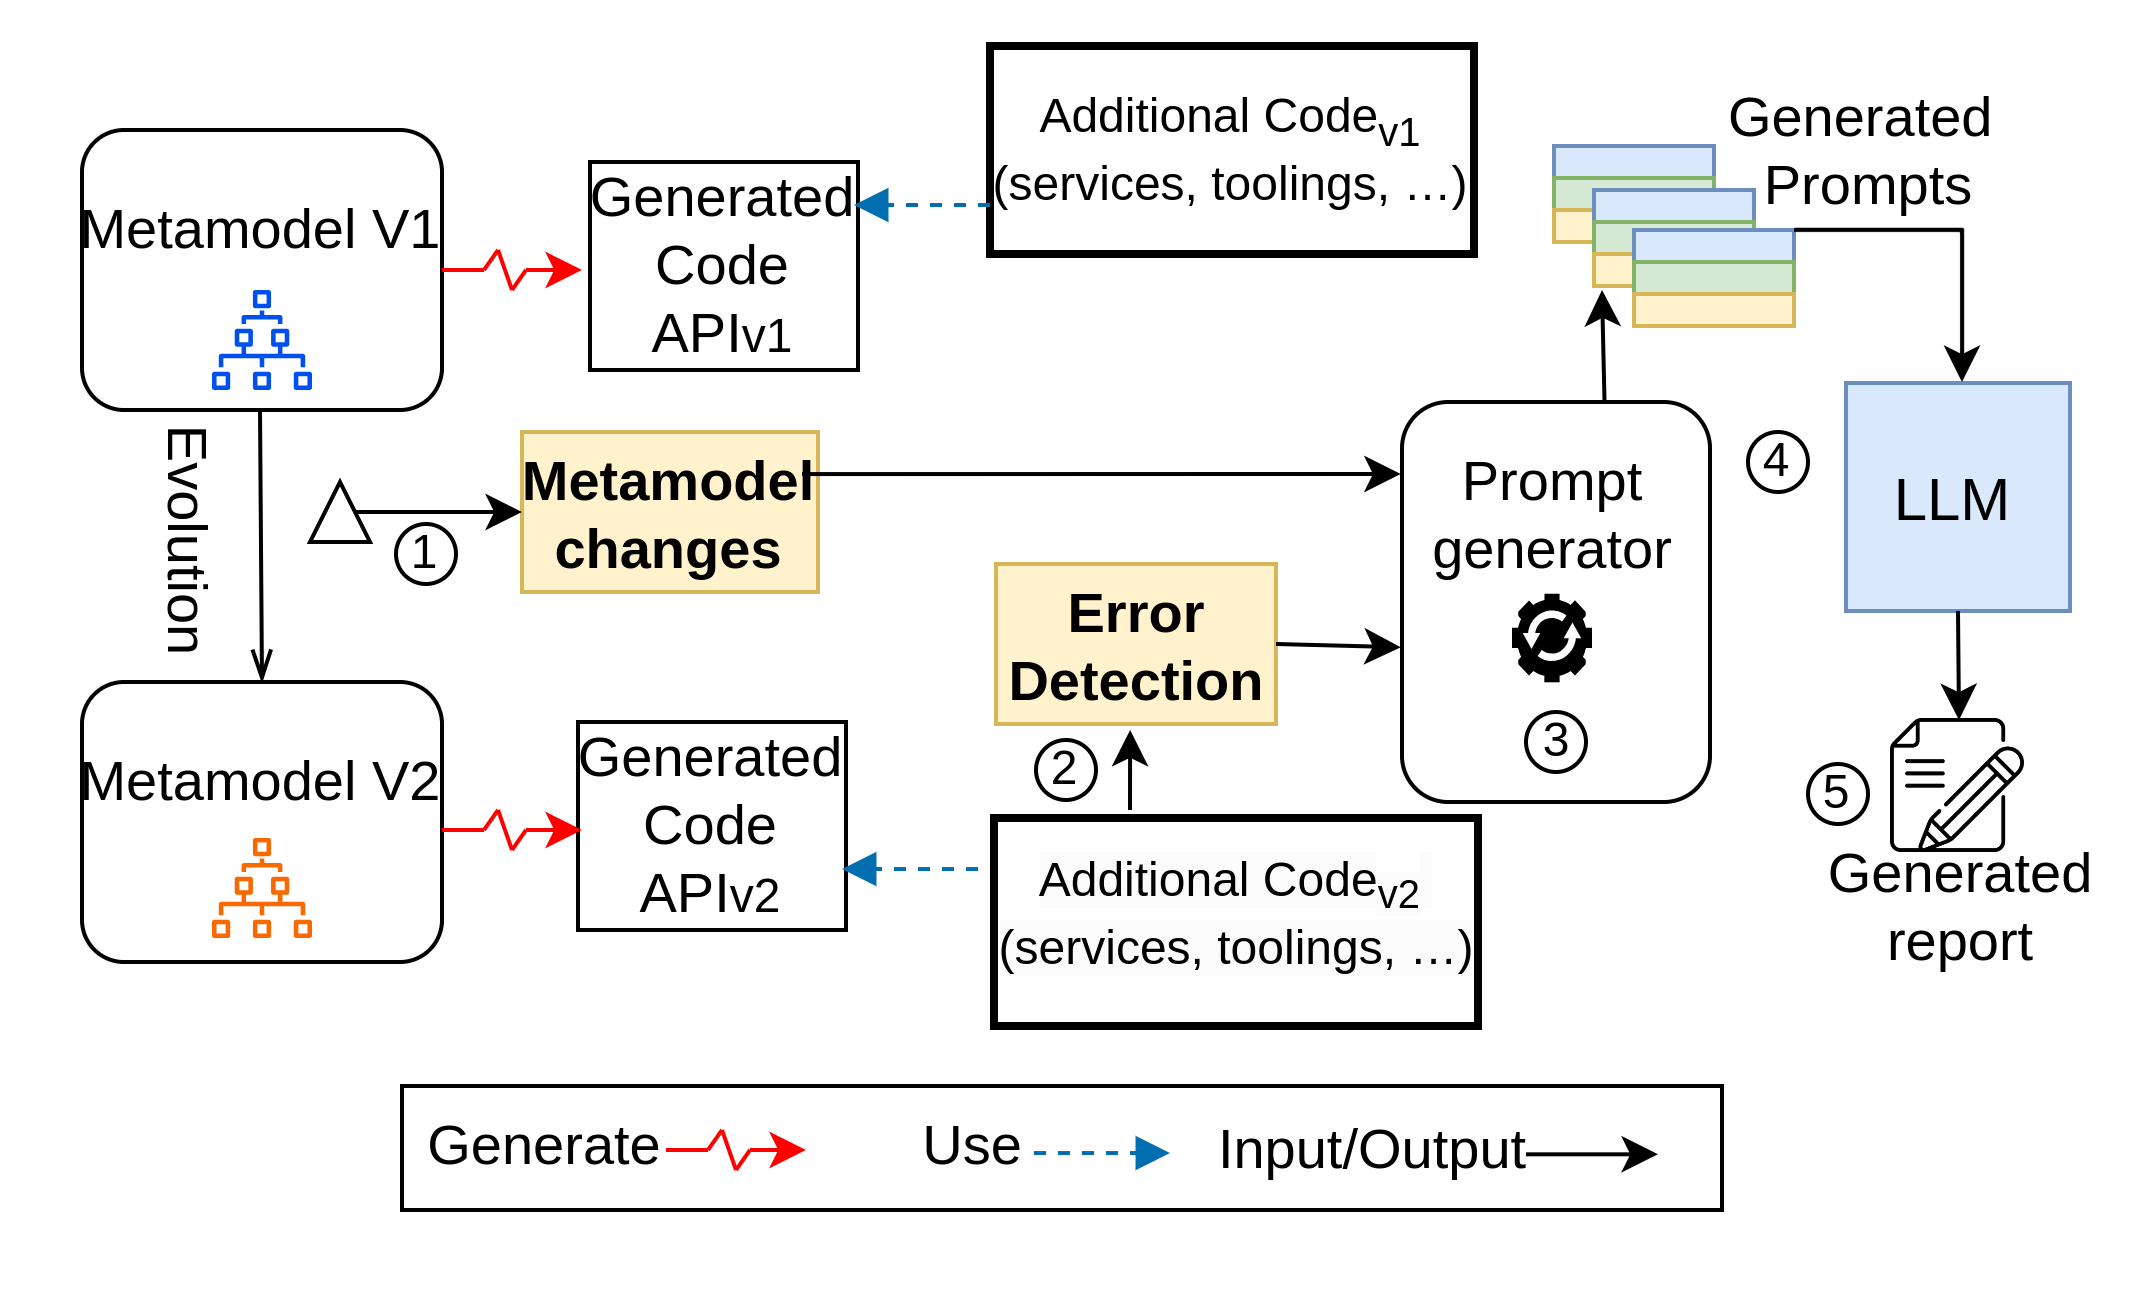
\includegraphics[width=0.7\textwidth]{./pics/chapter3pics/approach.png}
	\caption{Overall Approach for Prompt-based co-evolution.}
	\label{fig: approach}
	%\vspace{-5mm}
\end{figure}



\subsection{Overview}

Figure \ref{fig: approach} shows the overall steps of our approach. We start by retrieving the list of changes that describe the evolution between the old metamodel and the new metamodel~\Circled{1}. 

When the metamodel evolves, the code API is regenerated, therefore the additional code is broken. The additional code is then parsed to collect the list of errors~\Circled{2}. The list of changes and the list of errors are the inputs of our prompt generator. The goal is to generate a prompt for each error, including sufficient information about the change and the error itself~\Circled{3}.
Each generated prompt is used to request ChatGPT to give a correction for the concerned error~\Circled{4}. A global report is generated for the additional code to allow the developer to have a visual output about the generated prompts and the answers of the LLM~\Circled{5}. Algorithm \ref{algo:overallalgo} further depicts the overall method of co-evolution based on a given LLM. After we parse the project, we retrieve the list of errors per class (Lines 2-3). Then for each error, we generate the prompt (Lines 4-5) and call the LLM and record its co-evolution response for analysis (Lines 6-7).
%\Circled{1}


\begin{algorithm2e}[t]
	% \algsetup{linenosize=\tiny}
	\small
	\SetAlgoLined
	\KwData{EcoreModelingProject, changesList}
	javaClasses $\leftarrow$ Parse(EcoreModelingProject)
	
	\For {( jc $\in$ javaClasses)}
	{
		errorsList $\leftarrow $ getErrors(jc)
		
		\For{(error : errorsList)}
		{
			prompt $\leftarrow$ promptGenerator(error, changesList, jc)
			
			coevolutionResponse $\leftarrow$ callLLM(prompt)
			
			addToReport(error, prompt, coevolutionResponse)
		}
	}
	
	
	\caption{\LLM Co-evolution}
	\label{algo:overallalgo}
\end{algorithm2e}

\subsection{Generated Prompt Structure}

\begin{figure}[t]
	\centering
	%\hspace*{-1cm}
	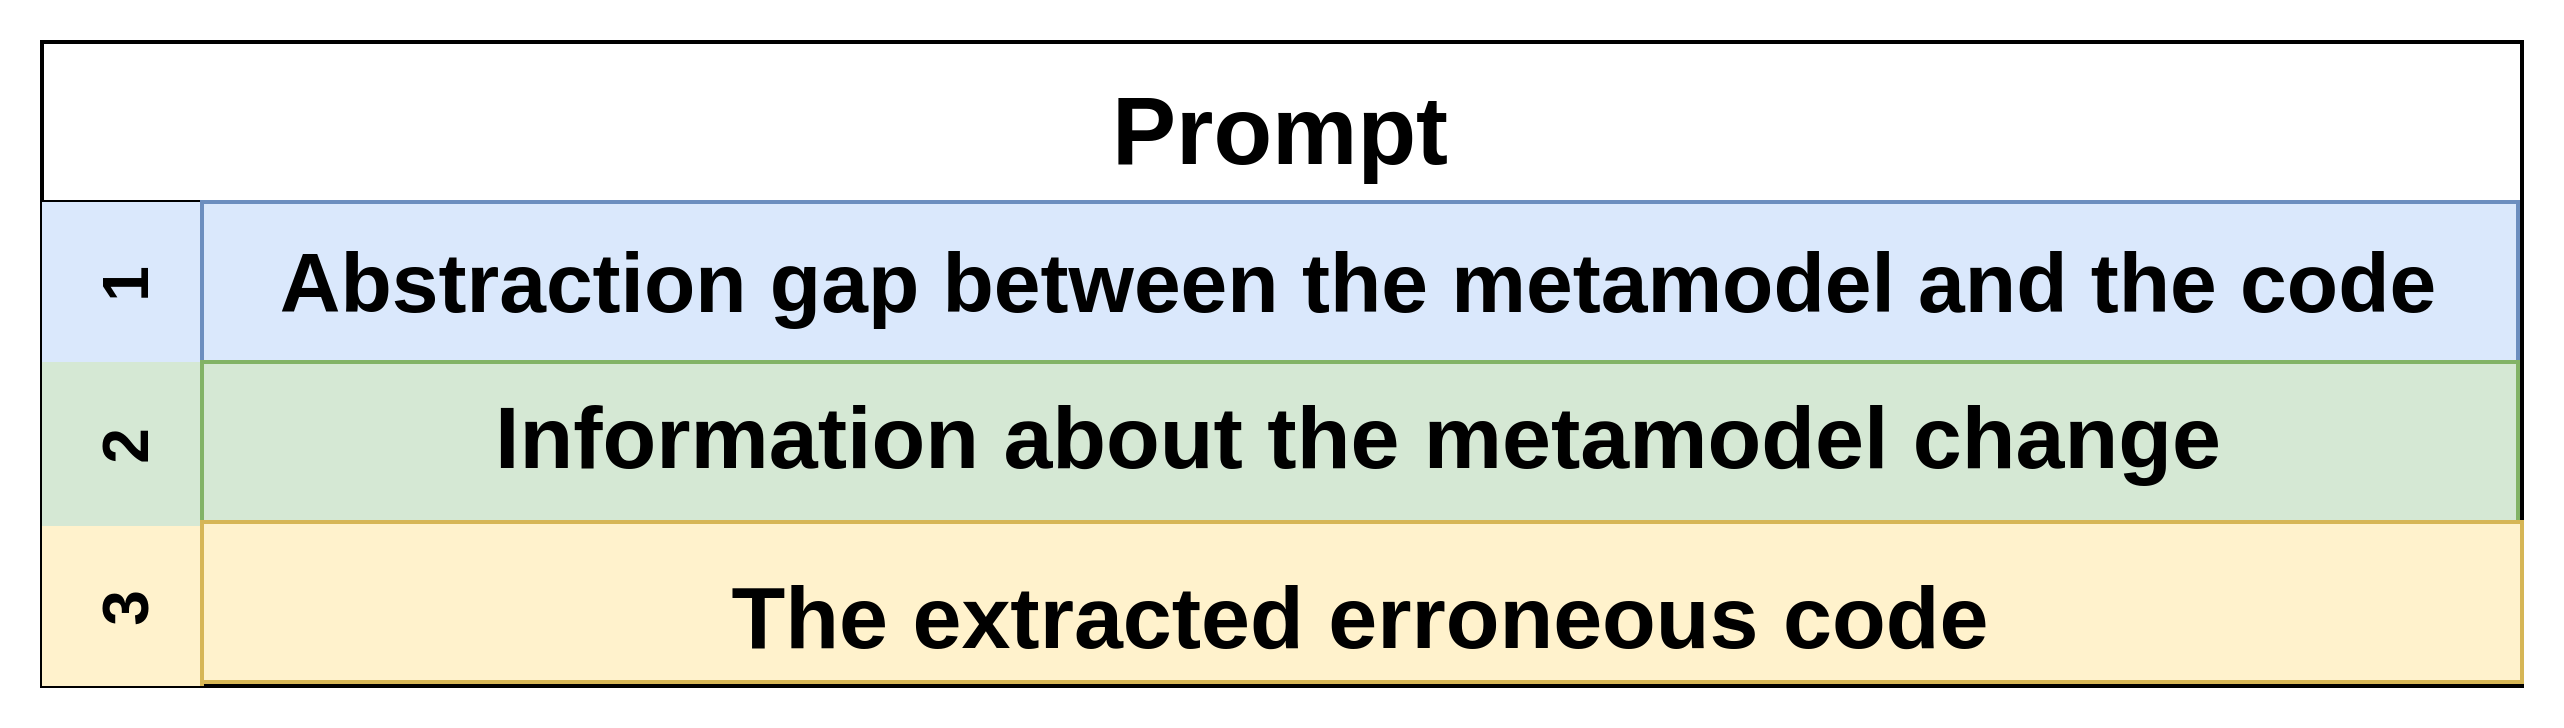
\includegraphics[width=0.65\textwidth]{./pics/chapter3pics/promptTemplate.png}
	\caption{Generated Prompt Structure.}
	\label{fig:promptstructure}
	\vspace{-5mm}
\end{figure}

Figure \ref{fig:promptstructure} shows the overall structure of the envisioned prompts we will generate in order to co-evolve the code errors. In fact, the rationale behind the prompt structure is that our problem does not only concern the code errors to repair, but it is also related to the use of the code generated from the metamodels and their changes. Therefore, to contextualize our problem, we must explain :~1) what is the code generated from the metamodels,~2) what is the impacting metamodel change, and~3) what is the impacted code error to co-evolve.  Concerning the prompt prefix we use "Co-evolve this code" to ask \LLM for one co-evolution. Next subsections detail the different parts of the prompt structure. 

\subsection{Abstraction Gap Between Metamodels and Code}

One main distinction from simply repairing code errors is the interplay between the metamodels and the additional code through the generated code from the metamodels. This is due to the gap in abstraction in between metamodels and generated code. In fact, for each metamodel various code elements are generated for each metamodel element and with different patterns.
Table~\ref{table:locationofMMelemen} classifies and provides illustrative examples for the different generated code elements from each metamodel element, namely metaclass, attribute/reference, and method.  %It shows that various code elements are generated for each metamodel element type and with different patterns. 
%%mapping between the different metamodel elements and their corresponding generated code elements with illustrative examples. 
For example, take the case of a metaclass\footnote{For simplicity, we refer to a metaclass by simply a class in the remaining of the chapter.}. EMF generates a corresponding interface and a class implementation, a \emph{createClass()} method in the factory class, three literals (\ie constants) for the class and an accessor method in the package class, and a corresponding to create adapter method. For the attribute case, EMF generates the signature and implementation of a getter and a setter, an accessor, and a literal. 
%This classification is essential to match the different errors with their corresponding pattern usages in the code, before to co-evolve them with the appropriate resolution strategy. 
This classification is essential to match the different errors with the right used generated code elements to explicit the abstraction gap. \red{If a class is changed, all its generated elements are impacted and their usages will be erroneous. For example, if a class is renamed, every invocation of the method "get+className" will be erroneous and must be co-evolved}. Thus, we consider the abstraction gap as the first contextual information we inject in the prompts for the LLM to co-evolve the code errors. 


\begin{table*}[t]

\caption{Classification of the different patterns of the generated code element from the metamodel elements. \\\hspace{3em} [Examples illustrated for a metaclass \emph{Rule}, property \emph{Status}, and method \emph{Execute()}]} 

\label{table:locationofMMelemen}
	\resizebox{17cm}{!} {
{\small
\begin{tabular}{llll}
\toprule

\begin{tabular}[c]{@{}l@{}} \textbf{Metamodel}\\ \textbf{element type} 
\end{tabular} & \textbf{Generated code elements}& \textbf{Pattern of the generated code elements}& \textbf{Examples}\\ \midrule


\multirow{6}{*}{Metaclass} & Interface & "MetaClassName" & \textit{Rule} \\ \cline{2-4} 
 & \begin{tabular}[c]{@{}l@{}}createClass() \\ (in metamodelFactory class)\end{tabular} & "create"+"MetaClassName"() &\textit{createRule()} \\ \cmidrule{2-4} 
 & \begin{tabular}[c]{@{}l@{}}Literals of the class \end{tabular} &
 \begin{tabular}[c]{@{}l@{}}
 "META\_CLASS\_NAME"\\
 "META\_CLASS\_NAME"+"\_"+ "FEATURE\_COUNT"\\
 "META\_CLASS\_NAME"+ "\_"+"OPERATION\_COUNT"
 \end{tabular} 
 & \begin{tabular}[c]{@{}l@{}}\textit{RULE}, \\ \textit{RULE\_FEATURE\_COUNT}, \\  \textit{RULE\_OPERATION\_COUNT}\end{tabular} \\ \cmidrule{2-4} 
 & \begin{tabular}[c]{@{}l@{}}Accessor of Meta objects \\ (in metamodelPackage class)\end{tabular} & "get"+"MetaClassName"()& \textit{getRule() }\\ \cmidrule{2-4} 
 & Class implementation & "MetaClassNameImpl" &\textit{RuleImpl }\\ \cmidrule{2-4} 
 & Adapter & "create"+"MetaClassName"+"Adapter" & \textit{createRuleAdapter()} \\ \midrule


\multirow{1}{*}{Attribute} & Signature of getters and setters & "get"+"AttributeName"(), "set"+"AttributeName"()& \textit{getStatus()}, \textit{setStatus() }\\ \cmidrule{2-4} 
\multirow{2}{*}{(Same for a} & Accessor of Meta objects &"get"+"MetaClassName"+"\_"+"AttributeName"() &\textit{getRule\_Status()} \\ \cmidrule{2-4} 
\multirow{1}{*}{Reference)}  & Literal & "META\_CLASS\_NAME"+"\_\_"+"ATTRIBUTE\_NAME"& \textit{RULE\_\_STATUS} \\ \cmidrule{2-4} 
 & \begin{tabular}[c]{@{}l@{}}Implementation \\ of getters and setters\end{tabular} &"get"+"AttributeName"(), "set"+"AttributeName"()& getStatus(), setStatus() \\ \midrule


\multirow{4}{*}{Method} & Declaration of the method& "methodName"()& \textit{Execute() }\\ \cmidrule{2-4} 
 & Accessor of meta objects &"get"+"MetaClass"+"\_\_"+"MethodName"()& \textit{getRule\_\_Execute() }\\ \cmidrule{2-4} 
 & Literal &"META\_CLASS\_NAME"+"\_\_"+"METHOD\_NAME"& \textit{RULE\_\_\_EXECUTE}\\ \cmidrule{2-4} 
 & Implementation of the method &"methodName"()& \textit{Execute()} \\ %\midrule


%\multirow{4}{*}{Reference} & Accessor of meta objects &"get"+"MetaClassName"+"\_"+"ReferenceName"()& \textit{getConstraint\_ConstraintElement()} \\ \cmidrule{2-4} 
% & Signature of getters and setter & "get"+"ReferenceName"(),"set"+"ReferenceName"()&\textit{ getConstraintElement()}, \textit{setConstraintElement() }\\ \cmidrule{2-4} 
% & Literal &"META\_CLASS\_NAME"+"\_\_"+"REFERENCE\_NAME"& \textit{CONSTRAINT\_\_CONSTRAINT\_ELEMENT} \\ \cmidrule{2-4} 
% & \begin{tabular}[c]{@{}l@{}}Implementation of \\ getters and setters\end{tabular} &"get"+"ReferenceName"(), "set"+"RegerenceName"()& \textit{getConstraintElement()}, \textit{setConstrainElement() }\\ 
\bottomrule
 
 %cline hline replaced with cmidrule and midrule
 
\end{tabular}
}
}
\end{table*}



\subsection{Metamodel Evolution Changes}
%\label{mmchanges}
The metamodel changes that we consider as the second contextual information, are injected in the prompts for the LLM to co-evolve the code errors. 

As a reminder, we use in this thesis a connection layer to our prompt generation approach.  This layer represents an interface specification of changes {\small\boxed{1}} bridging our prompt generator with the existing change detection approaches~\cite{Alter2015, williams2012searching,cicchetti_managing_2009,langer_posteriori_2013,vermolen_reconstructing_2012,Khelladi2016}.
Accordingly, we detail the changes that we consider in Table \ref{tab:changes}. 
%A metamodel represents a high abstraction level of a domain.
%Like any software artefact, metamodels evolve to meet domain changing requirements \cite{mens2008introduction}.
%Herrmannsdoerfer et al.~\cite{Herrmannsdoerfer2011} distinguish two types of metamodel changes: \emph{atomic} and \emph{complex}. Atomic changes are additions, removals, and updates of a metamodel element. Complex changes consist of a combination of atomic changes0~\cite{vermolen2011reconstructing,khelladi2015detecting}. 
%
%For example, push property is a complex change where a property is pushed from a parent class to an inheriting child class. This is composed of two atomic changes: delete a property and add a property~\cite{Herrmannsdoerfer2011}. 
%Many approaches in the literature~\cite{Alter2015, williams2012searching,cicchetti2009managing,langer2013posteriori,vermolen2011reconstructing,Khelladi2016,bettini2022executable} exist to detect metamodel changes between two versions. 
%\red{Particularly in our work, we use \cite{Khelladi2016,khelladi2016ad} to extract the changes between two metamodel versions. }

%In practice, we focus on the impacting metamodel changes that will require co-evolution of the code and not on the non-impacting changes. For example, an add change of a class does not require co-evolution. However, a delete change or a change of type will impact the code that must be co-evolved. 
%Table \ref{xyz} gives 
%The list of impacting metamodel changes \cite{iovino2012impact,cicchetti2009managing} we consider in the prompts is as follows: \emph{1)} Delete property\footnote{Property refers to Attribute, Reference, and Method.} \emph{p} in a class \texttt{C}, \emph{2)} Delete class \texttt{C}, \emph{3)} Rename element \emph{e} in a class \texttt{C}, \emph{4)} Generalize property \emph{p} multiplicity from a single value to multiple values in a class \texttt{C},  \emph{5)} Move property \emph{p} from class \texttt{Source} to \texttt{Target} through a reference \emph{ref},  \emph{6)} Extract class of properties $p_{1},...,p_{n}$ from \texttt{Source} to \texttt{Target} through a reference \emph{ref},  \emph{7)} Push property \emph{p} from super class \texttt{Super} to sub classes \texttt{Sub$_{1}$},...,\texttt{Sub$_{n}$}, \emph{8)} Inline class \texttt{Source} to \texttt{Target} with properties $p_{1},...,p_{n}$, and \emph{9)} Change property \emph{p} type from \texttt{S} to \texttt{T} in a class \texttt{C}. 

\begin{comment}
	\item \emph{1)} Delete property\footnote{Property refers to Attribute, Reference, and Method.} \emph{p} in a class \texttt{C}. 
	
	\item \emph{2)} Delete class \texttt{C}. 
	
	\item \emph{3)} Rename element \emph{e} in a class \texttt{C}. 
	
	\item \emph{4)} Generalize property \emph{p} multiplicity from a single value to multiple values in a class \texttt{C}. 
	
	\item \emph{5)} Move property \emph{p} from class \texttt{Source} to \texttt{Target} through a reference \emph{ref}. 
	
	\item \emph{6)} Extract class of properties $p_{1},...,p_{n}$ from \texttt{Source} to \texttt{Target} through a reference \emph{ref}. 
	
	\item \emph{7)} Push property \emph{p} from super class \texttt{Super} to sub classes \texttt{Sub$_{1}$},...,\texttt{Sub$_{n}$}. 
	
	\item \emph{8)} Inline class \texttt{Source} to \texttt{Target} with properties $p_{1},...,p_{n}$. 
	
	\item \emph{9)} Change property \emph{p} type from \texttt{S} to \texttt{T} in a class \texttt{C}. 
\end{comment}

%\emph{1)} Delete property \emph{p} in a class \texttt{C}. \emph{2)} Delete class \texttt{C}.\emph{3)} Rename element \emph{e} in a class \texttt{C}. \emph{4)} Generalize property \emph{p} multiplicity from a single value to multiple values in a class \texttt{C}. \emph{5)} Move property \emph{p} from class \texttt{S} to \texttt{T} through a reference \emph{ref}. \emph{6)} Extract class of properties $p_{1},...,p_{n}$ from \texttt{S} to \texttt{T} through a reference \emph{ref}. \emph{7)} Push property \emph{p} from super class \texttt{Sup} to sub classes \texttt{Sub$_{1}$},...,\texttt{Sub$_{n}$}. \emph{8)} Inline class \texttt{S} to \texttt{T} with properties $p_{1},...,p_{n}$. \emph{9)} Change property \emph{p} type from \texttt{S} to \texttt{T} in a class \texttt{C}.


\subsection{Extracted Code Errors}

Now that we have two main ingredients needed for the generation of the prompts. %, namely metamodel changes and the abstraction gap between metamodels and code. 
We only require the erroneous code to be co-evolved. 

To do so, we parse the code (i.e., \emph{compilation units}) to access the Abstract Syntax Trees (ASTs) and retrieve the code errors. %An error in a Java code is called a \emph{Marker} that contains the information regarding the detected error. It
Each error contains the necessary information to locate the exact impacted AST node in the parsed global AST (\ie char start and end) and to process it (\ie message). 
After that, we simply extract the sub-AST corresponding to the code containing the error. 
We consider three possible situations, namely 1) if the error is in a method, we extract the whole method, 2) if the error is in the imports, we extract the list of imports, 3) if the error is in the class definition or the fields, we extract it without the class's methods. This constitutes the final part of the contextual information we inject in the prompts for the LLM to co-evolve the code errors. Note that we simply specify in the prompt before the code the order to \emph{"Co-evolve this code: "}.
%\red{This prefix is selected after trying other terms like "update" and "correct" because it is more related to our problem.}.

%In the remaining part of the paper, we refer to errors and Java classes for the sake of simplicity. 


%\begin{figure}[t]\centering%
%\scalebox{0.9}{\small\input{pics/PromptStructure}}
% \vspace*{-0.3cm}
%\caption{Generated Prompt Structure.}
%\label{fig:promptStruct}
%\vspace{-1em}
%\end{figure}

\subsection{Prompt Generation}
\label{promptgeneration}

Algorithm~\ref{algo:promptgenerator} allows generating prompts following the specified structure in Figure~\ref{fig:promptstructure}. It first finds the ASTNode corresponding to the error in the code (Line~1). Then, it iterates over the list of metamodel changes to match  the error node with the code usage to identify the impacted abstraction gap (Lines~6-8). After that, it summarizes the impacting metamodel change (Line~11). Finally, it extracts the erroneous code (Line~21) and puts together all three contextual information into one generated prompt (Lines~22-25). 
%
Figure~\ref{fig:promptexample} shows an example of the generated prompt for the error in Listing~\ref{lis:Modisco_Code_External_V1} (Line~4) due to the move of property \emph{DiscoveryTimeInSeconds} in the metamodel.  

\begin{figure}[t]
	\centering
	%\hspace*{-1cm}
	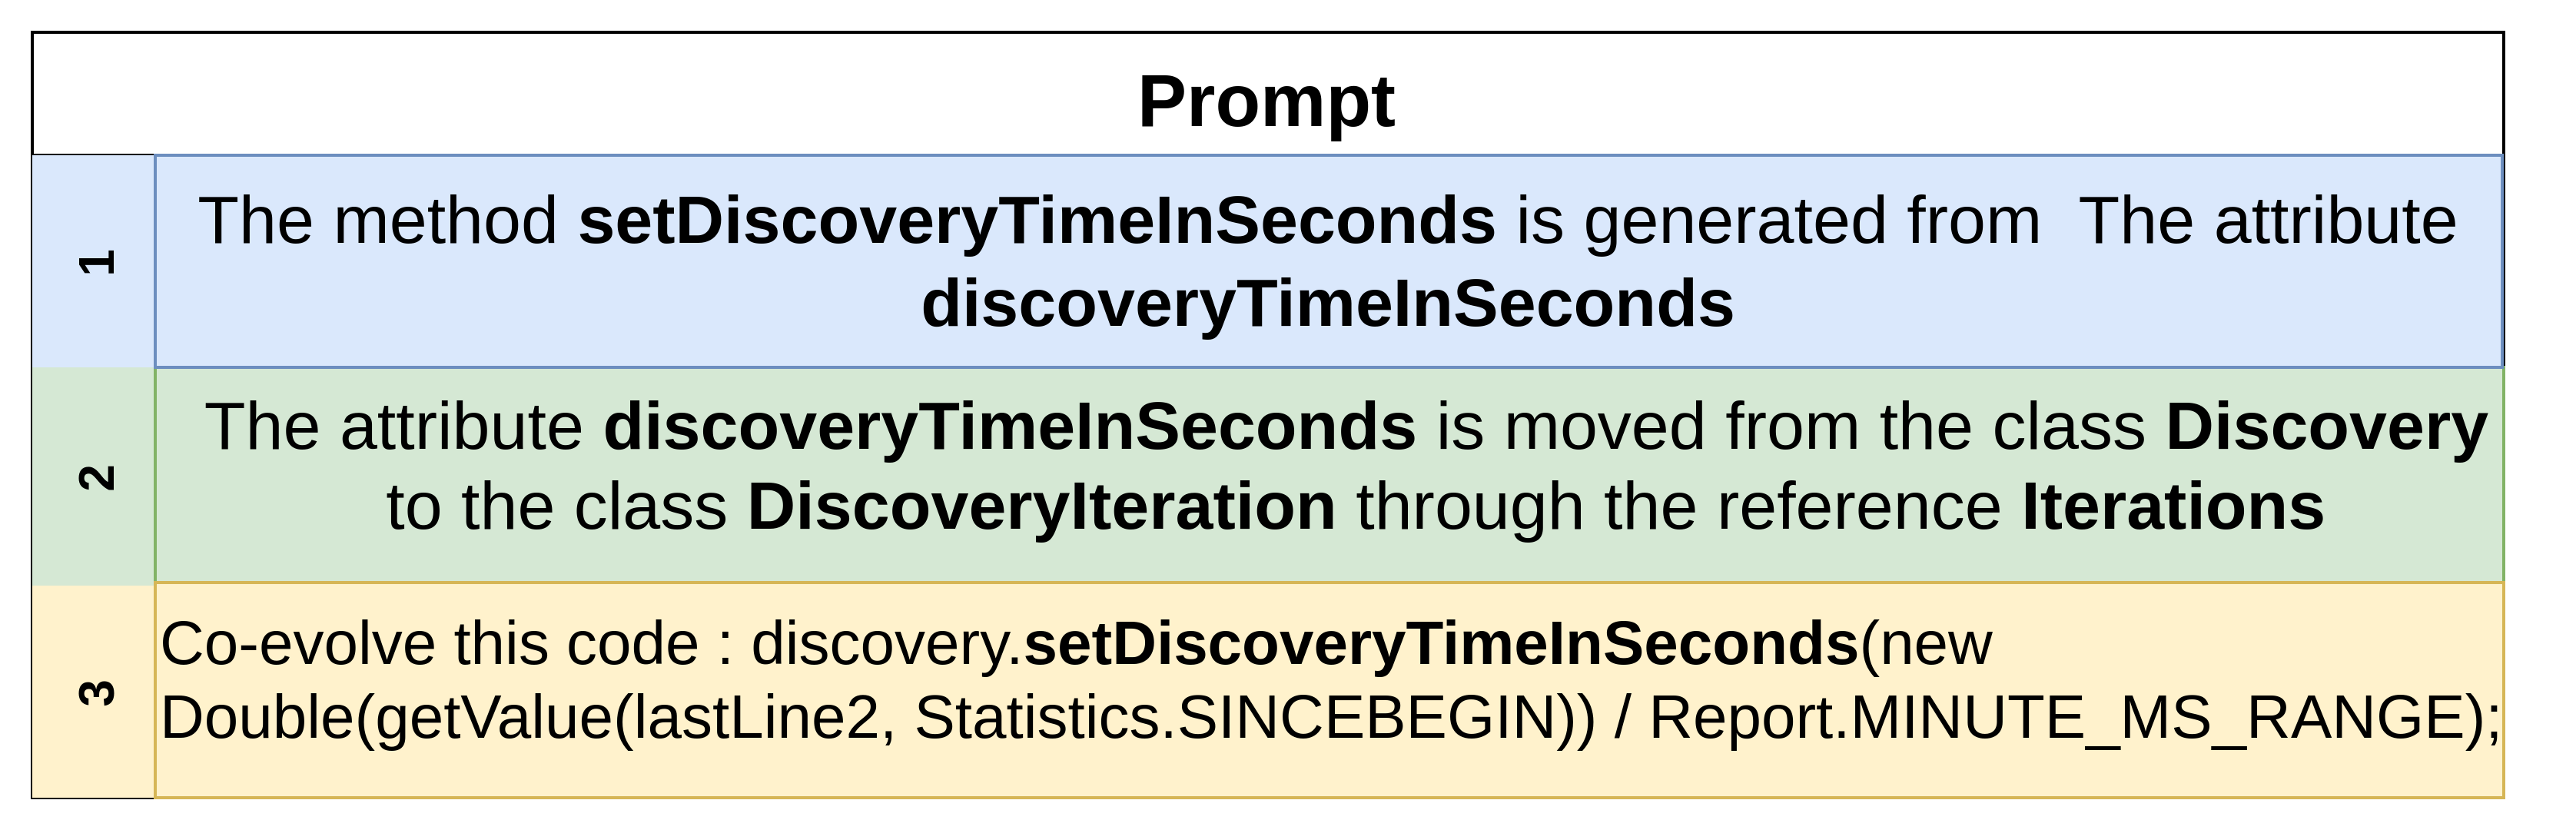
\includegraphics[width=0.5\textwidth]{./pics/chapter3pics/PromptStructure.png}
	\caption{Move attribute prompt example.}
	\label{fig:promptexample}
	\vspace{-5mm}
\end{figure}


\begin{algorithm2e}[t]
	% \algsetup{linenosize=\tiny}
	\small
	\SetAlgoLined
	\KwData{error, changesList, javaClass}
	
	errorNode $\leftarrow$ findErrorAstNode(javaClass, error)
	
	found $\leftarrow$ false
	
	%\uIf{(errornode.isTypeOf( SimpleName))}
	%{
		\While {(change  $\in$ changesList $\&$ $\neg found$)}
		{
			\Switch{change}{
				\Case{RenameClass}{%V errornode.name="set"+change.name)
					\uIf{(errornode.name="get"+change.name )}
					{
						found $\leftarrow$ true  
						
						abstractionGap="The method "+ errornode.name+" is generated from the metaclass "+ change.name
					} 
					\uElseIf {...}{\emph{\textcolor{circlegreen}{/*treat other abstraction gaps*/}}}
					changeInfo= "The metaclass "+ change.oldName+" is renamed to "+change.newName
				}
				\Case{RenameProperty}{
					...
				}
				\Case{DeleteProperty}{
					...
				}
			}
			
			
		}
		%} \uElseIf {( errornode.isTypeOf( QualifiedName))}
	%{	  \emph{\textcolor{circlegreen}{/*repeat same matching process*/}}
		%...
		%}
	
	
	codeError $\leftarrow$ extractCodeError(errornode)
	
	prompt.add(abstractionGap)
	
	prompt.add(changeInfo)
	
	prompt.add(codeError) 
	
	\textbf{return} prompt
	
	\caption{Prompt Generator Algorithm}
	\label{algo:promptgenerator}
\end{algorithm2e}


\begin{comment}
	
	
	\begin{algorithm2e}[t]
		% \algsetup{linenosize=\tiny}
		\small
		\SetAlgoLined
		\KwData{error, changesList, javaClass}
		
		errorNode $\leftarrow$ findErrorAstNode(javaClass, error)
		
		\uIf{(errornode.isTypeOf( SimpleName))}
		{
			\For {(change  $\in$ changesList)}
			{
				\Switch{change}{
					\Case{RenameClass}{%V errornode.name="set"+change.name)
						\uIf{(errornode.name="get"+change.name )}
						{
							request="The method "+ errornode.name+" is generated from the metaclass "+ change.name
							+" That is renamed from " +change.name+ " to "+change.newName
						}   
					}
					\Case{RenameProperty}{
						...
					}
					\Case{DeleteProperty}{
						...
					}
				}
			}
		} \uElseIf {( errornode.isTypeOf( QualifiedName))}
		{	  \emph{\textcolor{circlegreen}{/*repeat same matching process*/}}
			...
		}
		code$\leftarrow$getCode(errornode)
		
		prompt.add(request)
		
		prompt.add(code)
		
		\textbf{return} prompt
		\caption{Prompt generator algo}
		\label{algo:promptgenerator}
	\end{algorithm2e}
	
	
\end{comment}



%\subsection{Prototype Implementation}

\subsection{Prototype Implementation}
We implemented our solution as an eclipse Java plugin handling Ecore/EMF metamodels and their Java code. To retrieve the list of errors, we used JDT eclipse plugin \footnote{Eclipse Java development tools (JDT): \url{https://www.eclipse.org/jdt/core/}}. To launch our tool, we added a command to the context menu when selecting a java project. Generated prompts are sent to \LLM (see next section \ref{selectedLLM}), more specifically, its OpenAI API endpoint "https://api.openai.com/v1/chat/completions". We used Java JSON package to send our prompts and to receive \LLM responses. The error location, the corresponding generated prompt and \LLM responses are parsed in CSV file to have a visible results and to keep the history of proposed the co-evolutions.
Moreover, quick fixes (our baseline) are called using 
\textit{org.eclipse.jdt.ui.text.java.IQuickAssistProcessor} and \textit{org.eclipse.jdt.ui.text.java.IJavaCompletionProposal}.

\section{Methodology}
\label{ch3_evaluation}

This section describes our methodology for empirically assessing the capabilities of \LLM in addressing the problem of metamodel and code co-evolution. 
It first describes the selected LLM and the followed evaluation process.
Then, it presents our research questions and the data set.

\subsection{Selected LLM}\label{selectedLLM}
%\red(GPT-3.5, 4.0 ?)
% Motivate the use of chatgpt
% Motivate the use of gpt-3.5-turbo, chat mode

We chose to use \LLM \emph{GPT-3.5-turbo} in chat mode. It currently points to \emph{gpt-3.5-turbo-0613} released in June 2023. We opted for this model because of four factors. The first one is that prompt content is only textual, we don't need to inject audio or image content. The second one is its capacity to generate good answers for requests about code and models generation \cite{nathalia2023artificial,yeticstiren2023evaluating,guo2023exploring,fu2023chatgpt,kabir2023empirical,chaaben2023towards,camara2023assessment}. The third factor is that it was the latest API version that is accessible, \emph{gpt-4} API still not accessible for us. The last one is related to the high popularity of \LLM as a tool. It has more than 100 million users, and its website saw more than 1.7 billion visitors in the last three months, with Software and Software Development as visitors' top category\footnote{\url{https://www.similarweb.com/fr/website/chat.openai.com/\#demographics}}. 


\subsection{Evaluation Process}


First, as we aim to query \LLM to co-evolve the erroneous code due to metamodel evolution, we need to provoke the errors in the code. To do so, we replace the original metamodel by the evolved metamodel. Then, we regenerate the code API with EMF. This will cause errors in the additional code that must co-evolve. 
%
After that, we must map the errors with the causing metamodel change before to generate a prompt with all appropriate information to be able to co-evolve the code errors. We then rely on the OpenAI API to query \LLM before to analyze its results. 
%
%\todo{explain how we measure correctness ?}
%
Finally, we measure the correctness of \LLM co-evolution by comparing its co-evolution with the manually co-evolved version by developers. \red{Note that the comparison is processed manually by authors}. This allows us to measure the \emph{correctness} reached by \LLM. %We distinguish between \emph{syntactically} and \emph{semantically} correct co-evolution. The former is when \LLM gives the exact expected co-evolution that is also , whereas the latter is syntactically different but behave the same as the expected co-evolution, hence, semantically correct. 
%We consider a solution to be correct if it matches 
Correctness varies from~0 to~1, i.e., 0\% to 100\% and is defined as follows:
%alternative to terminology of syntactically, semantically
\vspace{0.5em}

\noindent $ Correctness = \dfrac{LLM Coevolutions \cap Manual Coevolutions}{Manual Coevolutions} $

\vspace{0.5em}

We chose the structure shown in Figure \ref{fig:promptstructure} since it contains the contextual information needed for our problem of metamodels and code co-evolution. \red{This structure was built after few manual naive attempts with \LLM, starting from a minimum context (as shown in the Motivating Example of Figure~\ref{fig: chatgptanswer} that failed) and by enriching the structure with more context information}. However, we do not claim its completeness in terms of needed information or if it is the best structure. Other variants can lead to different results. 
%for generated prompts after several manual attempts with Chatgpt. 
To investigate more this choice, we generated three more variations of this structure to observe its effect on the results. Table \ref{table: op variations} contains each variation and its corresponding explanation. Since our prompt contains three parts, we can change the order of these parts (Order Change operator) and the size of the erroneous code we put in the prompt (Minimal Code operator). Finally, rather than asking for a single co-evolution solution, we ask for alternative ones (Alternative Answers operator) in the prompt prefix. \red{To stress out our evaluation, we conducted 5 runs separated by almost a day, the time we needed for one run to check manually the results of each project, which means that each generated prompt is proposed to \LLM five times. This aims to check whether \LLM gives a same or different answer, hence, assess its robustness. 
	Finally, we compare \LLM to a baseline, namely the IDE quick fixes that are provided to repair the code errors. Note that we do not take as a baseline \LLM with prompts that only contain the code error, since as shown in Section \ref{ch3_example} and Figure \ref{fig: chatgptanswer}, it does not work. 
}


\subsection{Research Questions}

To assess the capabilities of \LLM in the co-evolution of code, we set the following research questions. 

\begin{itemize}
	\item[RQ1] %\subsubsection{RQ1} 
	%Can our code and metamodel coevolution appraoch using LLMs coevolve the code correctly? 
	To what extent can \LLM co-evolve the code with evolved metamodels? 
	This aims to assess the ability of \LLM to give correct resolutions to co-evolve the code according to the metamodel changes.
	
	\item[RQ2] %\subsubsection{RQ2}
	How does varying the temperature hyperparameter affect the output of the co-evolution? %How does our coevolution approach react to the variation of the prompt? 
	The temperature hyperparameter controls the creativity of the language model. 
	This question aims to assess the capability of \LLM to co-evolve the erroneous code when given less or more creativity in the generation of the solution. 
	
	
	\item[RQ3] %\subsubsection{RQ2}
	How does varying the prompt structure affect the output of the co-evolution? %How does our coevolution approach react to the variation of the prompt? 
	This aims to assess the quality improvement of the co-evolutions due to the prompts' variations.
	
	
	\item[RQ4] %\subsubsection{RQ3} 
	How does \LLM proposed co-evolution compare to the quick fix baseline? 
	As quick fixes are provided by default in an IDE to repair the code errors, this question aims to assess which method outperforms the other in the task of code co-evolution with evolving metamodels. %We measure its precision and recall and compare it with precision and recall of our automatic co-evolution approach.
	
	
\end{itemize}



\begin{table*}[t]
	\centering
	\caption{Variation operators of our original prompt (OP).}
	\label{table: op variations}
	\resizebox{14cm}{!} {
		\begin{tabular}{ll}
			\toprule
			Variation Operators       & Explanation                               \\ \midrule
			Order Change (OC)         & \begin{tabular}[c]{@{}l@{}}We change the order between the three structured parts of the prompt. \\  We start by describing  the metamodel change before the abstraction gap.\end{tabular} \\ \midrule
			Minimal Code (MC)         & \begin{tabular}[c]{@{}l@{}}Instead of giving the whole method that contains the code error to co-evolve, \\ we only give the instruction of code error.\end{tabular}     \\ \midrule
			Alternative Answers (AA)  & \begin{tabular}[c]{@{}l@{}}Instead of asking the LLM to give one solution of co-evolution, \\ we specifically ask for alternative ways to co-evolve the code error.\end{tabular}           \\
			\bottomrule
			
		\end{tabular}
	}
\end{table*}


\begin{table*}[t]
	\centering
	\caption{Details of the metamodels and their evolutions.}
	\label{CaseStudies_Evolution}
	\resizebox{16.5cm}{!} {
		\begin{tabular}{cllll}
			\toprule
			Case study                                                                            & \begin{tabular}[c]{@{}l@{}}Evolved \\ metamodels\end{tabular}                 & Versions & 
			\multicolumn{1}{c}{\begin{tabular}[c]{@{}c@{}}Atomic changes \\in the metamodel\end{tabular}} & \multicolumn{1}{c}{\begin{tabular}[c]{@{}c@{}}Complex changes \\in the metamodel\end{tabular}} \\ \midrule		
			
			
			OCL & \begin{tabular}[c]{@{}l@{}}Pivot.ecore in project\\ocl.examples.pivot\end{tabular}                        &  \begin{tabular}[c]{@{}l@{}}3.2.2 to\\ 3.4.4\end{tabular}        &   
			\begin{tabular}[c]{@{}l@{}} Deletes: 2 classes, 16 properties, 6 super types \\ Renames: 1 class, 5 properties \\ Property changes: 4 types; 2 multiplicities \\ Adds: 25 classes, 121 properties, 36 super types  \end{tabular}                                                         &    \begin{tabular}[c]{@{}l@{}} 1 pull property \\ 2 push properties  \end{tabular}                                                        \\ \midrule 
			Modisco & \begin{tabular}[c]{@{}l@{}}Benchmark.ecore in project\\modisco.infra.discovery.benchmark\end{tabular}                & \begin{tabular}[c]{@{}l@{}}0.9.0 to\\ 0.13.0\end{tabular}         &     
			\begin{tabular}[c]{@{}l@{}} Deletes: 6 classes, 19 properties, 5 super types \\ Renames: 5 properties  \\ Adds: 7 classes, 24 properties, 4 super types  \end{tabular}                                                        &     \begin{tabular}[c]{@{}l@{}} 4 moves property \\ 6 pull property \\ 1 extract class \\ 1 extract super class \end{tabular}                                                       \\ \midrule		
			
			
			Papyrus & \begin{tabular}[c]{@{}l@{}}ExtendedTypes.ecore in project\\papyrus.infra.extendedtypes\end{tabular}            & \begin{tabular}[c]{@{}l@{}}0.9.0 to\\ 1.1.0\end{tabular}         &   
			\begin{tabular}[c]{@{}l@{}}Deletes: 10 properties, 2 super types \\ Renames: 3 classes, 2 properies \\ Adds: 8 classes, 9 properties, 8 super types  \end{tabular}                                                      &    \begin{tabular}[c]{@{}l@{}} 2 pull property \\ 1 push property \\ 1 extract super class \end{tabular} \\  \bottomrule 		
		\end{tabular}
	}
\end{table*}



\begin{table*}[t]
	\caption{Details of the projects and their caused errors by the metamodels' evolution.}
	\label{CaseStudies_CoEvolution}
	\resizebox{18.5cm}{!} {
		\begin{tabular}{llcccccc}
			\toprule
			\begin{tabular}[c]{@{}l@{}}Evolved \\ metamodels\end{tabular}                 & \begin{tabular}[c]{@{}l@{}}Projects to co-evolve in response to the \\ evolved metamodels \end{tabular} 	& \begin{tabular}[c]{@{}c@{}}$N^{o}$ of \\ packages\end{tabular} & \begin{tabular}[c]{@{}c@{}}$N^{o}$ of \\ classes\end{tabular} & 
			\begin{tabular}[c]{@{}c@{}}$N^{o}$ of \\ LOC\end{tabular} & \begin{tabular}[c]{@{}c@{}}$N^{o}$ of Impacted \\ classes\end{tabular} & \begin{tabular}[c]{@{}c@{}}$N^{o}$ of total \\ errors \end{tabular}\\ \midrule		
			
			\begin{tabular}[c]{@{}l@{}}OCL  Pivot.ecore\end{tabular}                     
			& \begin{tabular}[c]{@{}l@{}} $[P1]$ ocl.examples.xtext.base \\ \end{tabular}   
			&   \begin{tabular}[c]{@{}l@{}}12 \end{tabular}    
			& \begin{tabular}[c]{@{}l@{}}181 \end{tabular}                 
			& 	\begin{tabular}[c]{@{}l@{}}17599 \end{tabular} 
			& \begin{tabular}[c]{@{}l@{}} 10 \end{tabular} 
			& \begin{tabular}[c]{@{}l@{}} 29 \end{tabular}
			\\ \midrule	
			\begin{tabular}[c]{@{}l@{}}Modisco \\ Benchmark.ecore\end{tabular}            
			& \begin{tabular}[c]{@{}l@{}} $[P2]$ modisco.infra.discovery.benchmark\\ $[P3]$ gmt.modisco.java.discoverer.benchmark\\ $[P4]$ modisco.java.discoverer.benchmark\\ $[P5]$ modisco.java.discoverer.benchmark.javaBenchmark\end{tabular}  
			& \begin{tabular}[c]{@{}l@{}}3 \\8 \\10 \\3  \end{tabular}
			& \begin{tabular}[c]{@{}l@{}}28 \\21 \\28 \\16 \end{tabular} 
			& \begin{tabular}[c]{@{}l@{}}2333 \\1947 \\2794 \\1654 \end{tabular} 
			& \begin{tabular}[c]{@{}l@{}}1\\4 \\9 \\9 \end{tabular} 
			& \begin{tabular}[c]{@{}l@{}}6 \\30 \\56 \\73 \end{tabular} 
			\\ \midrule		
			\begin{tabular}[c]{@{}l@{}}Papyrus \\ ExtendedTypes.ecore\end{tabular}          
			& \begin{tabular}[c]{@{}l@{}} $[P6]$ papyrus.infra.extendedtypes\\   $[P7]$ papyrus.uml.tools.extendedtypes\end{tabular}  & \begin{tabular}[c]{@{}l@{}}8 \\7 \end{tabular}
			& \begin{tabular}[c]{@{}l@{}}37 \\15  \end{tabular} 
			&\begin{tabular}[c]{@{}l@{}}2057  \\725  \end{tabular} 
			& \begin{tabular}[c]{@{}l@{}}8 \\7   \end{tabular}
			& \begin{tabular}[c]{@{}l@{}} 44\\28 \end{tabular} 
			\\ \bottomrule		
		\end{tabular}
	}
\end{table*}




\subsection{Data set}
\label{dataset}
This section presents the used data set in our empirical study, to be found in the attached supplementary material\footnote{\url{https://figshare.com/s/bf35039892799c0e6f34}}. 

We chose \red{Eclipse Modeling Framework (EMF) platform as technological space}, which allows us to build modeling tools and applications based on Ecore metamodels \cite{steinberg2008emf}. %This open source tool, is also adopted in industry, for instance, in SAP company\footnote{\url{https://help.sap.com/docs/SAP_POWERDESIGNER/1cc460ad80f446e6a9d19303919ee269/c7f1d7456e1b1014b1f5de4946b14e20.html?version=16.7.05}} thanks to its architecture and the tools it offers. It is actively updated, the last release was in November, 2023\footnote{\url{https://download.eclipse.org/modeling/emf/emf/builds/release/latest/index.html}}.    % \cite{ref?}. %In 2022, Eclipse IDE was downloaded 1 million times per month.
%
First, we aimed at selecting metamodels with meaningful \red{real} evolutions that do not consist in only deleting metamodel elements, but rather including complex evolution changes (see subsection \ref{mmchanges}). 

%By complex changes, we mean ....

This selection criterion resulted in seven Java projects from three case studies of three different language implementations in Eclipse, namely OCL~\cite{MDTOCL}, Papyrus \cite{MDTPapyrus}, and Modisco~\cite{MDTModisco} \red{with their versions that was manually co-evolved by developers, that represent our ground of truth}.
%
OCL is a standard language defined by the Object Management Group (OMG) to specify First-order logic constraints. Papyrus is an industrial project led by CEA\footnote{\url{http://www-list.cea.fr/en/}} to support model-based simulation, formal testing, safety analysis, etc. Modisco is an academic initiative to support development of model-driven tools, reverse engineering, verification, and transformation of existing software systems. 
%Papyrus is an industrial project led by CEA\footnote{\url{http://www-list.cea.fr/en/}} to support model-based simulation, formal testing, safety analysis, etc.  
Thus, the case studies cover standard, industrial, and academic languages that have evolved several times for more than 10 years of continuous development period.
%In particular, Papyrus and OCL are open source projects are actively maintained with frequent releases per year.

Table~\ref{CaseStudies_Evolution} presents the details on the selected case studies, in particular about their metamodels and the occurred changes during evolution. The total of applied metamodel changes was~330 atomic changes, including~19 complex changes in the three metamodels. 
%
Table~\ref{CaseStudies_CoEvolution} presents the details on the size of the seven projects and code of the original versions that we co-evolve in addition to the number of errors after the metamodels evolution. 

\section{Results}
\label{ch3__results}
This section now presents our results answering each RQ. 

\subsection{RQ1: Assessing the ability of \LLM to give correct code co-evolutions }

%execute with temp 0.2, single result, with whole method having the error, on many projects, 

%To what extent can \LLM co-evolve the code with metamodels? This aims 
To assess the ability of \LLM to give correct code co-evolutions, % the code according to the metamodel changes. 
%To answer this question, 
we ran over the errors caused by the metamodel changes and generated 266 prompts that we submitted to \LLM. 
Note that we ran our original prompts asking for a single co-evolution of the code error. We further set a fixed temperature hyperparameter to~0.2. A value of 0 restricts the generation of a solution towards a more deterministic one and the more it is higher the more creative the model gets in generating a different solution. Thus, we chose 0.2 to allow only little creativity while restricting the model to not get a different answer for the same prompts in different executions, since we ask for a single solution. 
%
Among the~266 generated prompts, \LLM gave, on average, a correct code co-evolution in~88.7\% of the time, varying from~75\% to 100\%. 
% \red{75\%} to \red{100\%}. 
\red{When taking only on complex changes into consideration, correctness improves on average from~88.7\% to~95.2\%, \ie \LLM performs better for complex changes.}
Results show a promising ability of \LLM to actually co-evolve code with evolving metamodels when given the right contextual information in the prompts, rather than simply the errors and their messages. 



\begin{table}
	\centering
	\caption{Measured correctness rate per temperature.}
	\label{table:correctnesspertemp}
	%\hspace*{-0.5cm}
	\resizebox{0.9\textwidth}{!} {
		\begin{tabular}{lllllllll}
			\toprule
			\centering
			& \multicolumn{6}{l}{\hspace{10.5em}\bfseries Projects}                                \\ %\cmidrule{3-7} 
			\multirow{3}{*}{\begin{turn}{-90}\bfseries Temperature\end{turn}} & \multicolumn{1}{l|}{}  & \multicolumn{1}{l|}{P1}       & \multicolumn{1}{l|}{P2}      &\multicolumn{1}{l|}{P3} & \multicolumn{1}{l|}{P4}   & \multicolumn{1}{l|}{P5}  & \multicolumn{1}{l|}{P6} & P7 \\ \cmidrule{2-9}
			
			& \multicolumn{1}{l|}{0.0} & \multicolumn{1}{l|}{76\%} & \multicolumn{1}{l|}{62.5\%}& \multicolumn{1}{l|}{100\%}& \multicolumn{1}{l|}{80\%}&\multicolumn{1}{l|}{86\%}&\multicolumn{1}{l|}{93.7\%}& 92.8\% \\ \cmidrule{2-9} 
			
			& \multicolumn{1}{l|}{0.2} & \multicolumn{1}{l|}{\cellcolor{green!35}\textbf{84\%}}& \multicolumn{1}{l|}{\cellcolor{green!35}\textbf{75\%}}& \multicolumn{1}{l|}{\cellcolor{green!35}\textbf{100\%}}& \multicolumn{1}{l|}{\cellcolor{green!35}\textbf{82\%}} &\multicolumn{1}{l|}{\cellcolor{green!35}\textbf{88\%}} &\multicolumn{1}{l|}{\cellcolor{green!35}\textbf{95.8\%}} & \cellcolor{green!35}\textbf{96.4\%} \\ \cmidrule{2-9} 
			
			& \multicolumn{1}{l|}{0.5} & \multicolumn{1}{l|}{57\%}& \multicolumn{1}{l|}{50\%}& \multicolumn{1}{l|}{100\%}& \multicolumn{1}{l|}{58\%} &\multicolumn{1}{l|}{68\%} &\multicolumn{1}{l|}{87.5\%} & 89.2\% \\ \cmidrule{2-9} 
			
			& \multicolumn{1}{l|}{0.8} & \multicolumn{1}{l|}{50\%}& \multicolumn{1}{l|}{37\%}& \multicolumn{1}{l|}{0\%}& \multicolumn{1}{l|}{32\%} &\multicolumn{1}{l|}{46\%} &\multicolumn{1}{l|}{62.5\%} & 85.7\% \\ \cmidrule{2-9} 
			
			& \multicolumn{1}{l|}{1.0} & \multicolumn{1}{l|}{30\%}& \multicolumn{1}{l|}{29\%}& \multicolumn{1}{l|}{0\%}& \multicolumn{1}{l|}{26\%} &\multicolumn{1}{l|}{40\%} &\multicolumn{1}{l|}{68.7\%} & 78.5\% \\ \bottomrule%\cmidrule{2-9} %
		\end{tabular}
	}
\end{table}


\begin{tcolorbox}[boxsep=-2pt]
	\textbf{$\boldsymbol{RQ_1}$ insights:}
	Results confirm that \LLM is able at 88.7\% to correctly co-evolve code due to metamodel evolution thanks to the information on the abstraction gap and the impacting metamodel change. It also performs better on complex changes.  
\end{tcolorbox}


\subsection{RQ2: Studying the impact of temperature variation on the output co-evolutions}
%execute with temp 0, 0.5, 0.8, 1.0

The temperature hyperparameter controls the creativity of the language model. The temperature hyperparameter in \LLM can be set between~0 and~2. Yet, it is suggested to only set it between~0 and~1 in the documentation\footnote{\url{https://platform.openai.com/docs/api-reference/chat}}. Thus, to assess the effect of the temperature in co-evolving the code, we will vary it on~0,~0.2,~0.5,~0.8,~and~1.0. 
Table \ref{table:correctnesspertemp} shows the obtained results. 

%How does varying the temperature hyperparameter affect the output of the co-evolution? %How does our coevolution approach react to the variation of the prompt? 

%This question aims to assess the capability of \LLM to co-evolve the erroneous code when given less or more creativity in the generation of the solution. 
%we observe that the more we increase the temperature, the less correct are the code co-evolutions that are suggested by
Overall, we observe that as the temperature increases, the correctness of code co-evolutions suggested by \LLM decreases. Notably, the correctness improves when the temperature is increased from~0 to~0.2. However, it subsequently degrades with the further increase in temperature, up to~1. At temperatures~0.8 and~1, we observed the worst decrease in correctness. % does not exceed~50\% and~40\%, respectively. 
The best performance of \LLM is obtained at the temperature~0.2. Note that even with a temperature set to~0, which implies no creativity, \LLM yields results that are nearly as satisfactory as those obtained with a temperature of~0.2.

\red{Moreover, when we repeated the same prompt for each temerature for 5 times, the five answers of \LLM were similar. \LLM gives almost the same proposition of co-evolution, sometimes it uses different terms to comment its answer. For example: \textit{"// Remove the following line since DiscoveredProject is removed"} and \textit{" // Code using DiscoveredProject should be removed"}. However, they are the same co-evolutions. Sometimes \LLM also uses intermediate variables to give the same co-evolution, for example:\textit{ "return aReport.generate()"} and \textit{benchmarkModel=aReport.generate() return benchmarkModel"}. 
	We believe that this result of obtaining the same co-evolutions over 5 runs shows the efficiency of the prompt template in Figure~\ref{fig:promptstructure}. 
	By including the necessary information (i.e., abstraction gap, causing change information, and code error), it allows \LLM to narrow the scope of possibilities and to propose similar answer for each unique prompt in each run.}

\begin{tcolorbox}[boxsep=-2pt]
	\textbf{$\boldsymbol{RQ_2}$ insights:}
	Results show that lower temperature of~0 and~0.2 give better co-evolutions from \LLM with~0.2 being the best we observed. 
	Interestingly, we obtained the same results over 5 different runs, which suggests the efficiency our prompt structure in narrowing the scope of possibilities of \LLM's answers. 
\end{tcolorbox}


\subsection{RQ3: Studying the impact of prompt structure variation on the output co-evolutions}
%Execute prompts starting by the gap information followed by the change information then 

%by starting by the change followed by the gap

%execute prompt with minimal code (instruction)

%??? execute prompt with less code (surrounding instruction) ???
%??? execute prompt without abstraction gap ???

%execute prompt while asking for many alternative solutions

%How does varying the prompt affect the output of the co-evolution? %How does our coevolution approach react to the variation of the prompt? 
In our approach, we propose a possible structure for the generated prompts (cf. Subsection \ref{promptgeneration}). However, there is no assurance that this represents the best proposition. Therefore, we varied the structure that we proposed in three different ways, as shown in Table \ref{table: op variations}.  Then we ran the three variations of the original prompts in order to assess the fluctuation and effect on the correctness of the proposed co-evolutions. Here we set the temperature to 0.2 based on results of RQ2. % due to the variation of the prompt. 

%we can of course vary them, which in turn can affect the correctness of the proposed co-evolutions. 
%To assess the quality improvement of the proposed resolutions due to the variation of the prompt. We ran the experiments with three additional variations of our original prompts, as shown in Table \ref{table: op variations}. 

%\red{Table \ref{x} shows xyz relevant prompt variations in our context of metamodels and code co-evolution that we will assess.}


\begin{table}
	\centering
	\caption{Measured correctness rate for different prompt variations. [$\nearrow$ and  $\searrow$ are increase and decrease in correctness.]}
	\label{table:correctnessVariation}
	\hspace*{-0.5cm}
	\resizebox{0.7\textwidth}{!}{ 
		
		\begin{tabular}{lllllllll}
			\toprule
			\centering
			& \multicolumn{8}{l}{\hspace{15.5em}\bfseries Projects}                                \\ %\cmidrule{3-7}
			\multirow{3}{*}{\begin{turn}{-90}\bfseries Variations\end{turn}} & \multicolumn{1}{l|}{}  & \multicolumn{1}{l|}{P1}       & \multicolumn{1}{l|}{P2}      &\multicolumn{1}{l|}{P3} & \multicolumn{1}{l|}{P4}  &\multicolumn{1}{l|}{P5}  &\multicolumn{1}{l|}{P6}  & P7 \\ \cmidrule{2-9}
			
			%& \multicolumn{1}{l|}{\begin{tabular}[c]{@{}l@{}}Original \\ Prompt (OP)\end{tabular}} & \multicolumn{1}{l|}{84\%} & \multicolumn{1}{l|}{75\%}& \multicolumn{1}{l|}{100\%}& \multicolumn{1}{l|}{82\%}& \multicolumn{1}{l|}{88\%}& \multicolumn{1}{l|}{95.8\%}& 96.4\% \\
			%\cmidrule{2-9} 
			
			& \multicolumn{1}{l|}{\begin{tabular}[c]{@{}l@{}}Original \\ Prompt (OP)\end{tabular}} & \multicolumn{1}{l|}{\textbf{84\%}}& \multicolumn{1}{l|}{\textbf{75\%}}& \multicolumn{1}{l|}{\textbf{100\%}}& \multicolumn{1}{l|}{\textbf{82\%}} &\multicolumn{1}{l|}{\textbf{88\%}} &\multicolumn{1}{l|}{\textbf{95.8\%}} & \textbf{96.4\%} \\ \cmidrule{2-9} 
			
			& \multicolumn{1}{l|}{\begin{tabular}[c]{@{}l@{}}Order \\ change (OC)\end{tabular}} & \multicolumn{1}{l|}{84\%}& \multicolumn{1}{l|}{\cellcolor{red!15}66\%$\searrow$}& \multicolumn{1}{l|}{100\%}& \multicolumn{1}{l|}{\cellcolor{red!15}74\%$\searrow$} &\multicolumn{1}{l|}{\cellcolor{red!15}86\%$\searrow$} &\multicolumn{1}{l|}{95.8\%} & 96.4\% \\
			\cmidrule{2-9} 
			
			& \multicolumn{1}{l|}{\begin{tabular}[c]{@{}l@{}}Minimal \\ Code (MC)\end{tabular}} & \multicolumn{1}{l|}{\cellcolor{green!35}88.4\%$\nearrow$}& \multicolumn{1}{l|}{\cellcolor{green!35}87.5\%$\nearrow$}& \multicolumn{1}{l|}{100\%}& \multicolumn{1}{l|}{\cellcolor{green!25}86\%$\nearrow$} & \multicolumn{1}{l|}{\cellcolor{green!35}96\%$\nearrow$} & \multicolumn{1}{l|}{\cellcolor{green!25}97.9\%$\nearrow$} & 96.4\% \\
			\cmidrule{2-9} 
			
			& \multicolumn{1}{l|}{\begin{tabular}[c]{@{}l@{}}Alternative \\ Answers (AA)\end{tabular}} & \multicolumn{1}{l|}{84\%}& \multicolumn{1}{l|}{\cellcolor{green!25}79\%$\nearrow$}& \multicolumn{1}{l|}{100\%}& \multicolumn{1}{l|}{\cellcolor{green!35}92\%$\nearrow$} & \multicolumn{1}{l|}{\cellcolor{green!25}92\%$\nearrow$} &\multicolumn{1}{l|}{95.8\%} &96.4\%\\ \bottomrule %\cmidrule{2-7} %
			%\cellcolor{green!35}$\searrow$
			%\textcolor{red}{$\searrow$} \textcolor{green}{$\nearrow$}
			
		\end{tabular}
	}
\end{table}


Table \ref{table:correctnessVariation} shows the obtained results. Overall, we observe slight increase and decrease compared to the original Prompts structure~(\textbf{OP}). 
We observe that changing the order in the prompt by first describing the metamodel change (\textbf{OC}) decreases the correctness of the proposed \LLM co-evolutions. It decreased by~-9\% in P2,~-8\% in P4 and by~-2\% in P5. We observed that in particular when describing the abstraction gap with the generated elements for the metamodel deleted classes, % information in the case of deletions, 
\LLM assumes that the code classes still exist in the code and were not deleted. Thereby, altering sometimes the correctness of its proposed co-evolutions. 

However, the two other prompt variations of giving a minimal code containing the error and asking for alternative solutions delivered better overall results. 
Surprisingly, on the one hand, giving only the code instruction containing the error (\textbf{MC}) gave the best results. It improved by~+4.4\% in P1,~+12.5\% in P2,~+4\% in P4, ~+8\% in P5, and ~+2.1\% in P6. 
Our observation is that this improvement is sometimes due to the inability of \LLM to find the impacted code element and co-evolve it within complex and long methods. 
On the other hand, when asking for alternatives, it improved only by~+4\% in P2,~+10\% in P4, and~+4\% in P5. We observed that when \LLM is unable to find the correct resolution with (\textbf{OP}) prompts, it is unlikely to find the right one when asking for alternatives (\textbf{AA}). Only in few cases it could find the correct co-evolutions.  %We noticed also that 
The generation of prompts and saving the results took on average from about~10 seconds per prompt for the Original Prompts to~84 seconds per prompt in the case of Alternative Answers (AA) variation prompts.
\red{Finally, when focusing only on complex changes, correctness improves on average from 88.7\% to 97.6\% for \textbf{(MC)} and \textbf{(AA)}. This implies that, overall, \LLM also performs better for complex changes when varying the prompts. This can be explained by the fact that complex changes provide much more context information that guide better \LLM to give better responses.} 
%on  the variation operator



\begin{tcolorbox}[boxsep=-2pt]
	\textbf{$\boldsymbol{RQ_3}$ insights:}
	Results show an improvement with two variants out of the three we explored. However, gains are not significant compared to our original structure of the prompt. 
	Variants also perform better on complex changes. 
\end{tcolorbox}

\subsection{RQ4: Comparison with quick fixes as baseline}
%230441
%compare with quick fixes

%How does \LLM proposed co-evolution compare to the quick fix baseline? 
%As quick fixes are provided by default in an IDE to repairs the code errors, this question aims to assess which method outperform in the task of code co-evolution with evolving metamodels.

To compare to a baseline the obtained results of proposed co-evolutions with our generated prompts, we checked what is the best quick fix an IDE proposes for each error. Algorithm~\ref{algo :quickfixes} shows the followed steps to run the quick fixes on our projects automatically. 
It iterates over the java classes and for each error, we  automatically apply the top quick fix suggested by the IDE. 
It stops when all the errors disappear or if the remaining errors have no possible quick fixes purposed by the IDE. 
%It stops in three cases : 1) if all the errors disappear, or 2) if the remaining errors have no possible quick fixes, or 3) the application of a quick fix causes an infinite loop \cite{cuadrado2018quick,khelladi2019detecting}, i.e., a cycle of applying a quick fix that causes a previously fixed error~(~A $\mapsto$ ~B $\mapsto$ ~A $\mapsto$ ~B $\mapsto$ ...). 

In Table~\ref{AppliedQF}, we present the percentage of errors that quick fixes eliminated for each project. %, and the frequencies of each type of applied quick fixes. 
%
While the quick fixes eliminated from~41\% to~100\% errors. We use the term eliminated instead of correct co-evolution because no quick fix was applied as expected to the manual developers' co-evolutions. In other words, the correctness rate of automatic quick fixes are equal to 0 and are not suited for the task of metamodels and code co-evolution.
For example, concerning errors caused by class or property deletion from the metamodel, renaming a class or an attribute, moving, pushing or pulling attributes or methods from a class to another, the quick fixes proposed to create them back in their old containers. This is in contradiction of the applied metamodel changes and the code co-evolution.  

For errors caused by changing a variable's type, the quick fixes always proposed to add a cast with a wrong type. 

Similarly, as naive prompts with only the code errors and their messages, quick fixes do not take in consideration the knowledge of the abstraction gap and the information contained in its causing metamodel changes. For example, the quick fix \texttt{create the missing method \emph{m()}} is applied no matter the metamodel change (i.e., deletion, moving, pulling, or pushing changes) and no matter the metamodel element it was generated from.
Our approach of generated prompts takes into account the context of the impacted code, the abstraction gap, and the causing metamodel change thanks to the prompt template that we designed (cf. Table \ref{fig:promptstructure}).

\begin{tcolorbox}[boxsep=-2pt]
	\textbf{$\boldsymbol{RQ_4}$ insights:}
	Results show that \LLM with our generated prompts completely outperforms the quick fixes in correctly co-evolving the code. 
\end{tcolorbox}




\begin{algorithm2e}[t]
	% \algsetup{linenosize=\tiny}
	\small
	\SetAlgoLined
	\KwData{EcoreModelingProject}
	javaClasses $\leftarrow$ Parse(EcoreModelingProject)
	
	\For {( jc $\in$ javaClasses)}
	{
		errorsList $\leftarrow $ getErrors(jc)
		
		\While{(!errorsList.isEmpty() \& hasQuickFix)}
		{
			error  $\leftarrow$ errorsList.next()
			
			\uIf {error.hasQuickickFix() }
			
			{
				useQuickFixes(error) %\COMMENT{Eclipse quick fix}
			}
			
			
			refreshJavaClass(jc) 
			
			refreshErrorsList(jc, errorsList)
		}
		
	}
	
	\caption{Quick fixes for coevolution}
	\label{algo :quickfixes}
\end{algorithm2e}



\begin{table}[t]
	\centering
	\caption{Number of applied Quick Fixes for each project and per evolved metamodel.}
	\label{AppliedQF}
	\resizebox{0.7\textwidth}{!} {
		\begin{tabular}{lll}%ll}
		\toprule
		\begin{tabular}[c]{@{}l@{}}Evolved \\ metamodels\end{tabular} & \begin{tabular}[c]{@{}l@{}}Co-evolved \\ projects\end{tabular}  & \begin{tabular}[c]{@{}l@{}} \% of eliminated \\ errors  \end{tabular} %& \begin{tabular}[c]{@{}l@{}} $N^{o}$ of applied \\ Quick Fixes \end{tabular}  & Total
		\\ \midrule 
		\begin{tabular}[c]{@{}l@{}}OCL Pivot.ecore\end{tabular}
		
		& $[P1]$ & 41\% 
		%&\begin{tabular}[c]{@{}l@{}} $ [ $Create method $] $: 4,$[ $Change to m' $] $:11,\\     $ [ $change type of var or return type $] $: 1,\\     $ [ $Add unimplemented methods $] $: 2,     \end{tabular}  & 18
		\\ \midrule			
		\multirow{4}{*}{\begin{tabular}[c]{@{}l@{}}Modisco \\ Benchmark.ecore\end{tabular}}  &  $[P2]$& 100\%
		%& \begin{tabular}[c]{@{}l@{}}  
		%  $[ $  $] $     $[ $ Create Class X  $] $: 6,  $[ $ Add unimplemented methods  $] $: 1    \end{tabular}  & 7
	\\ \cmidrule{2-3}			
	
	& $[P3]$ &100\% 
	%& \begin{tabular}[c]{@{}l@{}}    $[ $ Create Class X $] $: 2,$[ $  Create method $] $: 8,\\ $[ $ Change m to m' $] $; 5, $[ $ Remove argument $] $: 1,\\ $[ $ Add cast $] $ : 6   \end{tabular}  & 22
	\\ \cmidrule{2-3}			
	
	& $[P4]$ &83\%
	%& \begin{tabular}[c]{@{}l@{}}     $[ $  Create Method $] $: 17,  $[ $ Change method m to m' $] $: 16, \\ $[ $ Remove argument $] $: 2,  $[ $ Change type of var or return type $] $: 1,\\  $[ $ Add Cast$] $: 16.    \end{tabular}& 52 
	\\ \cmidrule{2-3}			
	
	& $[P5]$&67\% 
	%& \begin{tabular}[c]{@{}l@{}} $[ $ Change method m to m' $] $: 4, $[ $ Add unimplemented methods  $] $: 2,\\ $[ $ Create Constant$] $:9, $[ $ change type $] $ : 2,\\$[ $ Add Cast  $] $: 6    \end{tabular}& 23  
	\\ \midrule			
	
	\multirow{2}{*}{\begin{tabular}[c]{@{}l@{}}Papyrus \\ ExtendedTypes.ecore\end{tabular}} &  $[P6]$&69\%
	%& \begin{tabular}[c]{@{}l@{}}     $[ $ Create Class X $] $: 3,  $[ $ Create method m $] $: 9,\\  $[ $ Change method m to m' $] $: 13,  $[ $Change type of var or return type  $] $: 5, \\$[ $ Add Cast $] $: 4,  $[ $Add unimplemented methods$] $: 2.   \end{tabular} & 36
	\\ \cmidrule{2-3}			
	
	
	&  $[P7]$ &93\% 
	
	%\begin{tabular}[c]{@{}l@{}}     $[ $ Create Class X $] $: 1,  $[ $ Create method $] $ : 14,\\ $[ $ Create Constant $] $ :3,  $[ $ Add Cast$] $: 2,\\  $[ $ Change method m to m' $] $:3.   \end{tabular} & 23
	\\ %\midrule			
	%Total &&&& 429 \\ 
	\bottomrule
	
	
\end{tabular}  

}
%\hspace{1em}
\end{table}

\subsection{Threats to Validity}
This section discusses threats to validity w.r.t. Wohlin et al. \cite{wohlin2012experimentation}.

\subsubsection{Internal Validity.} 
%internal => prompt engineering?? only vary temperature, choice of API Mode completion (our choice) vs Chat

A first internal threat is that we only varied the temperature hyperparameter over \LLM API. The documentation suggests not to modify top\_p and temperature at the same time, so we chose to let the default value of top\_p =~1. 
Moreover, to measure the correctness, we analyzed the developers' manual co-evolution.
To mitigate the risk of misidentifying a manual co-evolution, for each impacted code error, we mapped it in the co-evolved class version. If we did not find it, we further searched in other classes in case the original impacted part of the code was moved into another class. Thus, our objective was to reduce the risk of missing any mappings between an error in the original code and its co-evolved version. Moreover, as our co-evolution relies on the quality of detected metamodel changes. We also validated each detected change by checking whether it occurred between the original and evolved metamodels. This alleviates the risk of relying on an incorrect metamodel change that would degrade the generated prompts and lead to wrong co-evolution from \LLM. 
%Note that the order of changes taken as input does not influence our co-evolution, but the order of errors we treat may affect the distribution of the applied resolutions. However, we took the order in which the errors were detected. 
%\red{Finally, to reduce risk of getting random answers from \LLM, we ran 5 times the evaluation and the prompts. It showed that our results are robust and that the capability of \LLM in co-evolving code is not due to randomness.} 

\subsubsection{External Validity.}
%external => cannot generalize to other LLMs such as Lamma, => future work to replicate

We implemented and ran the empirical study for EMF and Ecore metamodels and Java code. Note that \red{the choice of Java is imposed by EMF and no other languages are supported. Thus, we naturally do not generalize to other languages.} 
We also relied only on \LLM and GPT-3.5-turbo released in june~2023. 
Therefore, we cannot generalize our approach to other LLMs and other future versions of \LLM. It is also unclear how our findings would transfer to other benchmarks other than EMF Ecore metamodels and java code. Further experiments are necessary in future to get more insights and- before any generalization claims.  


\subsubsection{Conclusion Validity.}
%conclusion => do we have significant results 

Our empirical study show promising results with \LLM being able to generate correct code co-evolution when given the necessary contextual information. It showed to be useful, with an average of~88.7\% correctness (from~75\% to~100\%). The results also show the benefit over relying on quick fixes. Nonetheless, even though we evaluated it on real evolved projects, we must evaluate it on more case studies to have more insights and statistical evidence.  %further evaluation is needed on more case studies.

\subsection{Discussion and Limitations}
The rationale behind the prompt structure, which an important part in our empirical study, is that our problem concerns the use of the code generated from the metamodels and their changes and not only error repair. Moreover, our results show that \LLM can co-evolve the code correctly by setting lower temperature, especially in case of complex metamodel changes. Furthermore, repeating the experimentation five time has led to the same results shown in Table \ref{table:correctnesspertemp} and Table \ref{table:correctnessVariation}, which confirms the robustness of \LLM in the code co-evolution task and that his capability is not due to randomness.
Finally, we handled a single metamodel with changes that are independent between them. Treating the case of multiple metamodel and the case of interdependent changes would need setting an order of priority between them, which we left for a future work.
%Overall, our findings contribute to a deeper understanding of \LLM ability in the metamodel and code co-evolution context
%say it works well, remind bets results,  => it could replace quick fixes

%then discuss limitation 1) des LLMs for co-evolution  2) of our prompts 


\section{Conclusion}
\label{ch3_conclu}
%write conclu here later \todo{Djamel}
Co-evolving the impact of metamodel evolution on the code is costly and yet challenging. In this chapter, we propose a prompt-based approach for metamodel and code co-evolution. This approach relies on designing and generating a rich contextual information that we inject in the prompts, namely the abstraction gap knowledge, the metamodel changes information and  the impacted code to be co-evolved.
We evaluated our approach on seven EMF projects and three evolved metamodels from three different Eclipse EMF implementations of OCL, Modisco and Papyrus, with a total of~5320 generated prompts. Results show that on average \LLM has successfully proposed~88.7\% of correct co-evolutions with our original generated prompts. We evaluated then the impact of the temperature variation on the proposed co-evolutions. We found that \LLM gives better responses with lower temperature values of~0 and~0.2. 
Moreover, when experimenting other variations of the structure of generated prompts, we observed that there was improvement in two variations. 
%The first one is changing the order of the contextual information in the prompt, and the second one is requiring alternative answers for the co-evolution. Varying the prompt by giving only a minimum code to co-evolve degraded the quality of the proposed co-evolutions. 
The first one is giving the minimum impacted code to co-evolve in the prompt, and the second one is requiring alternative answers for the co-evolution. However, varying the prompt by changing the order of the contextual information degraded a little the quality of the proposed co-evolutions. 
Finally, we compared our approach with the quick fixes of the IDE as a baseline. Results show that our approach significantly outperforms the quick fixes that do not take into account the context of the abstraction gap and the metamodel changes.

%As future work, we intend to evaluate or approach in other technological spaces than EMF, such as OpenAPI and the challenge of the API evolution impact on clients' code. After that, we plan to transform our approach into a DSL-based approach with a graphical user interface for the output report instead of a CSV file. To facilitate prompt generation and enhance the option of prompt variation, a DSL would be a viable solution. We also plan to replicate our empirical study with other LLMs and other contexts of co-evolution (e.g., between code and test \cite{le2021untangling}).  Another actionable element is to investigate the mining of contextual information from Software Engineering tasks to enrich the prompts, and then improve baseline results
%Finally,\red{ since our contributions focus on empirically studying the use of \LLM in metamodel and code co-evolution, we plan to implement an alternative of the quick fix engine in the Eclipse IDE based on our generated prompt structure. Integrating our prompt-based metamodel and code co-evolution in the IDE will have a direct impact in helping MDE developers and language engineers}. 


